\chapter[Absorbing Sets of Array-based LDPC Codes]{Absorbing Sets of Array-based LDPC
Codes}\label{arrayabs}

In this Chapter we provide a detailed analysis of the  minimal
absorbing sets and minimal fully absorbing sets of the high rate
array-based LDPC codes.

\section{Array-based LDPC Code Construction}

Array based LDPC codes \cite{fan} are regular LDPC codes
parameterized by a pair of integers $(\gamma, p)$, such that
$\gamma \leq p$, $p$ is an odd prime, with a parity check matrix
$H_{p,\gamma}$ given by
\begin{equation}\label{eq:1}
H_{p,\gamma}=\left[\begin{array}{ccccc}
I & I & I & \ldots & I\\
I & \sigma & \sigma^2 & \ldots &\sigma^{p-1}\\
I & \sigma^2 & \sigma^4 & \ldots &\sigma^{2(p-1)}\\
\vdots & \vdots & \vdots & \ldots & \vdots \\
I & \sigma^{\gamma-1} & \sigma^{(\gamma-1)2} & \ldots &\sigma^{(\gamma-1)(p-1)}\\
\end{array}
\right]
\end{equation}\normalsize
where $\sigma$ denotes a $p \times p$ permutation matrix of the
form \small
\begin{equation}
\sigma=\left[\begin{array}{ccccc}
0 & 0 & \ldots & 0 & 1\\
1 & 0 & \ldots & 0 & 0\\
0 & 1 & \ldots & 0 & 0\\
\vdots & \vdots & \ldots & \vdots & \vdots\\
0 & 0 & \ldots & 1 & 0\\
\end{array}
\right].
\end{equation}
\normalsize We use $C_{p,\gamma}$ to denote the binary linear code
with the parity check matrix (\ref{eq:1}).

As demonstrated in \cite{fan}, array-based LDPC codes have very
good performance. They have been proposed for a number of
applications, including digital subscriber lines \cite{ibm:02} and
magnetic recording  \cite{vasic:05}.




\section{Theoretical Results}\label{theo1}

Our goal is to describe minimal absorbing sets and minimal fully
absorbing sets $(a,b)$ of the Tanner graph of the parity check
matrix $H_{p,\gamma}$, for $\gamma =2,3,4$, where the minimality
refers to the smallest possible $a$, and where $b$ is the smallest
possible for the given $a$.

We use the following notation throughout the Chapter. For
$H_{p,\gamma}$ viewed as a two-dimensional array of matrices, we
let $j$ for $0 \leq j \leq p-1$ be the column-wise index in
$H_{p,\gamma}$ and call it the column group $j$, and we let $i$
for $0 \leq i \leq \gamma-1$ be the row-wise index in
$H_{p,\gamma}$ and we call it the row group (or the label) $i$.
Let $G_{p,\gamma}$ be the Tanner graph associated with
$H_{p,\gamma}$ (bit nodes and check nodes in $G_{p,\gamma}$
represent columns and rows in $H_{p,\gamma}$, respectively). Each
bit node $\ell$ in $G_{p,\gamma}$ is uniquely indexed by
$(j_\ell,k_\ell)$ where $j_\ell$ denotes the column group of the
corresponding column, and $k_\ell$, $0 \leq k_\ell \leq p-1$,
denotes the index of that column within the column group $j_\ell$
it belongs to. Each check node in $G_{p,\gamma}$ receives a label
$i$ if it belongs to the row group $i$. Multiple check nodes can
have the same label.

We note that the structure of the parity check matrix imposes the
following conditions on the neighboring bit nodes and check nodes:

\textit{Vertex Consistency:} For a bit node, all its incident
check nodes, labelled $i_{s_1}$ through $i_{s_\gamma}$ must have
distinct labels, i.e. these check nodes are in distinct row
groups.

\textit{Edge Consistency:} All bit nodes, say $(j_{d_1},k_{d_1})$
through $(j_{d_p},k_{d_p})$, participating in the same check node
must have distinct $j_\ell$ values, i.e. they are all in distinct
column groups.

Both conditions follow from the fact that the parity check matrix
$H_{p,\gamma}$ of $C_{p,\gamma}$ consists of a 2-dimensional array
of circulant matrices of equal size.

Our main results can be summarized as follows: Let $G_{p,\gamma}$
be the Tanner graph associated with the parity check matrix
$H_{p,\gamma}$ of the array-based LDPC code $C_{p,\gamma}$.
\begin{theorem}\label{theo1}\emph{Minimality}

(a) For the $G_{p,2}$ family, all minimal absorbing sets are
minimal fully absorbing sets and are of size $(4,0)$.

(b) For the $G_{p,3}$ family, the minimal absorbing sets are of
size $(3,3)$, and the minimal fully absorbing sets are of size
$(4,2)$.

(c) For the $G_{p,4}$ family, and for $p>19$, all minimal fully
absorbing sets are minimal absorbing sets, and are of size
$(6,4)$.\hfill$\blacksquare$
\end{theorem}
\begin{theorem}\label{theo2}\emph{Scaling}

(a) Suppose $\gamma=2$ and $p>3$. The number of minimal (fully)
absorbing sets in $G_{p,\gamma}$ grows with block length $n$
($n=p^2$ is the number of columns in $H_{p,\gamma}$) as
$O(n^{2})$.

(b) Suppose that either $\gamma =3$ and $p
>3$ or $\gamma=4$ and $p > 19$. Then the number of minimal absorbing sets as well
as the number of minimal fully absorbing sets in $H_{p,\gamma}$
grows with block length $n=p^2$ as $O(n^{3/2})$.
\hfill$\blacksquare$
\end{theorem}

The following three subsections provide proofs of these claims,
where we separately treat each of the values of $\gamma$.

\subsection{Absorbing sets of
$H_{p,2}$}\label{theo12}

The code $C_{\gamma,2}$ has uniform bit degree 2, and is thus a
cycle code. Even though such codes are known to be poor, we
include the analysis for the sake of completeness.
%\begin{lemma}\label{Lemma02} The minimal absorbing set for $C_{p,2}$
%is if of dimension $(4,0)$.
%\end{lemma}
We start by proving the statement in Theorem~\ref{theo1}(a).
%\noindent \textit{Proof:}
\comment{ It follows from the definition of the absorbing set that
all $a$ bit nodes must be connected to satisfied checks with
respect to the subgraph induced by these bit nodes. The minimal
absorbing set thus corresponds to the support of a minimum weight
codeword. Since $\gamma=2$, Massey's theorem \cite{lincostel}
guarantees that $d_{min} \geq 4$. We first show that the smallest
cycle in this code is of length 8. We note that a cycle of length
4 cannot exist, as it would imply the existence of $\sigma^{j_1}$
and $\sigma^{j_2}$, for $0 \leq j_1, j_2 \leq p-1$ and $j_1 \neq
j_2$ that contain the same row. (Recall that the top row of
$H_{p,\gamma}$ consists of a row of identity matrices.) This
set-up is impossible by the code construction. For the same
reason, nor does there exist a cycle of length 6. We now show that
$a=4$ and these bit nodes complete an 8-cycle with their shared
check nodes. }

Let $G_{p,2}=(V,F,E)$ denote the Tanner graph of $H_{p,2}$. Let
$D$ be an $(a,b)$ absorbing set in $G_{p,2}$. Each bit node in $D$
has degree $2$ in $G_{p,2}$ and is required to have strictly more
neighbors in $\mathcal{E}(D)$ than in $\mathcal{O}(D)$. This
implies that $\mathcal{O}(D)$ is empty. The absorbing set is of
type $(a,0)$. It is thus a fully absorbing set, and is in fact a
codeword.

Since the matrix $H_{p,2}$ has top row consisting of identity
matrices, the codewords of $C_{p,2}$ are of even weight. Moreover,
$a>2$ since no two columns of $H_{p,2}$ sum to zero. Thus $a \geq
4$.

Let $(j_1,k_1)$, $(j_2,k_2)$, $(j_3,k_3)$ and $(j_4,k_4)$ be the
bit nodes participating in a $(4,0)$ absorbing set, which must
necessarily be as in Fig.~\ref{Fig03}, since there are no cycles
of length 4.
\begin{figure}
\center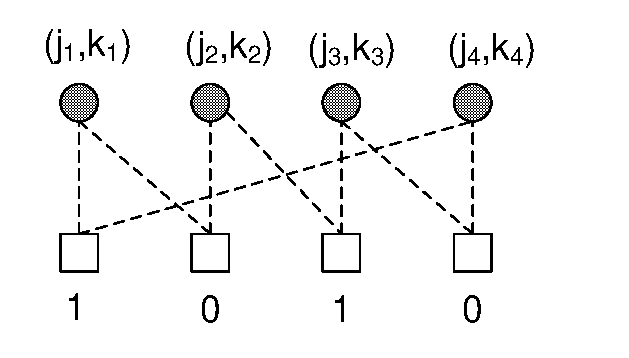
\includegraphics[width=2.75in,height=1.4in]{fig03.eps}
\caption{(Labelled) candidate (4,0) absorbing set}\label{Fig03}
\end{figure}
%By the vertex consistency condition, all the bit nodes that share
%a check node have different first indices. We may thus assume that
%$(j_1,k_1)$ and $(j_2,k_2)$ share a check in the row group $0$, as
%do $(j_3,k_3)$ and $(j_4,k_4)$, and that $(j_2,k_2)$ and
%$(j_3,k_3)$ share a check in the row group $1$, as do $(j_4,k_4)$
%and $(j_1,k_1)$, as shown in Fig. \ref{Fig03}.
Consider the matrix $M$,
\begin{equation}
M=(\sigma^{0j_1})^T(\sigma^{0j_2})(\sigma^{1j_2})^T(\sigma^{1j_3})(\sigma^{0j_3})^T(\sigma^{0j_4})(\sigma^{1j_4})^T(\sigma^{1j_1}).
\end{equation}

\noindent This matrix $M$ has a non-zero entry on the main
diagonal, and since it is itself a power of $\sigma$, it is
necessary that $M=\sigma^{p\ell}$, for some $\ell$, where $\ell$
is an integer.

Moreover, since
\begin{equation}\label{eq1}
(\sigma^{\ell})^T=(\sigma^{\ell})^{-1} \end{equation} it further
follows that
\begin{equation}\label{eq1}
p\ell=j_3-j_2+j_1-j_4.
\end{equation}

\comment{One solution to the last equation is $\ell = 0$, and
$j_1=1, j_3=p-1, j_2=2, j_4=p-2$. Since $(j_1,k_1)$ and
$(j_2,k_2)$ share a check in the row group $0$, it follows that
$k_1=k_2$, and likewise $k_3=k_4$. Since the column $k_2$ of
$\sigma^{j_2}$ and column $k_3$ of $\sigma^{j_3}$ have a non-zero
entry in the same row, it follows that
\begin{eqnarray*}
k_2+j_2 &\equiv & k_3+j_3 \mod p.
\end{eqnarray*}

Thus, the indices of the bit nodes participating in one such
absorbing set are $(j_1,k_1)$, $(j_2,k_1)$, $(j_3,[k_1-p+3]_p)$,
and $(j_4,[k_1-p+3]_p,)$, for $k_1$ chosen arbitrary in the
residue set$\mod p$, and where $[x]_p$ here and in the remainder
denotes a residue congruent to $x\mod p$.\hfill$\blacksquare$}

%It can be checked that for $\gamma=2$ the indicator function of
%every absorbing set is a codeword.
%\begin{lemma} The total number of $(4,0)$ absorbing sets in $C_{p,2}$ is XXXXX.
%\end{lemma}
%\noindent \textit{Proof:} It suffices to consider $l=-1,0,1$ in
%\ref{eq1}). First, for $l=0$ there are \hfill$\blacksquare$


\begin{lemma}\label{lemma40} There is a total of $p^2(p-1)^2$ $(4,0)$ (fully) absorbing sets in
the code described by $H_{p,2}$.
\end{lemma}
\noindent \textit{Proof:} It suffices to consider $\ell=1,0,-1$ in
(\ref{eq1}).

First, for $\ell=1$, there are $(s+1)(p-s-1)$ ways of assigning
values to $(j_1,j_2,j_3,j_4)$ to make $j_2+j_4=s$ and
$j_1+j_3=p+s$, for $0 \leq s \leq p-2$. Thus, \[\sum_{s=0}^{p-2}
(s+1)(p-s-1)=p(p-1)(p+1)/6\] is the total number of ways of
assigning values to $(j_1,j_2,j_3,j_4)$. By symmetry, for
$\ell=-1$ there are also $p(p-1)(p+1)/6$ ways of assigning values
to $(j_1,j_2,j_3,j_4)$.

For $\ell=0$, for each $s$, $0 \leq s \leq p-1$, there are $s+1$
ways of expressing $s$ as a sum of an ordered pair. For $s$ odd,
each of these $s+1$ ordered pairs can be assigned to $(j_1,j_3)$,
and for each such assignment, $s-1$ ordered pairs can be assigned
to $(j_2,j_4)$ (here $j_1 \neq j_2,j_4$ and $j_3 \neq j_2,j_4$ by
the edge consistency). For $s$ even, for $s$ assignments out of
possible $s+1$ (excluding the pair $(s/2,s/2)$) of $(j_1,j_3)$,
$s-1$ ordered pairs can be assigned to $(j_2,j_4)$. For the pair
$(s/2,s/2)$ assigned to $(j_1,j_3)$, there are $s$ available
assignments for $(j_2,j_4)$. For $p-1 \leq s \leq 2p-2$ the number
of assignments is the same as for $2p-2-s$. The total number of
assignments for $l=0$ is \[2\sum_{s=1,s \text{odd}}^{p-2}
(s+1)(s-1) + 2\sum_{s=2,s \text{even}}^{p-3} i^2 + (p-1)^2 =
2p(p-1)(p-2)/3~.\]



The total number of assignments for $(j_1,j_2,j_3,j_4)$ is then
$p(p-1)^2$. Since the column $k_1$ of $\sigma^{1j_1}$ and the
column $k_4$ of $\sigma^{1j_4}$ have a non-zero entry in the same
row, it follows that
\begin{equation}
k_1+j_1 \equiv k_4+j_4 \mod p~.
\end{equation}
Likewise,
\begin{equation}
k_2+j_2 \equiv k_3+j_3 \mod p~,
\end{equation}
\begin{equation}
k_1 \equiv k_2 \mod p~, and
\end{equation}
\begin{equation}
k_3 \equiv k_4\mod p~.
\end{equation}

Therefore, once the values of  $(j_1,j_2,j_3,j_4)$ are selected,
$k_1$ can be chosen in $p$ ways, and for each such assignment, the
values of $k_2$, $k_3$, and $k_4$, are then uniquely determined.
Hence, there are $p^2(p-1)^2$ different $(4,0)$ (fully) absorbing
sets.\hfill$\blacksquare$

\begin{corollary} The number of $(4,0)$ (fully) absorbing sets for
the code described by $H_{p,2}$ is $O(n^{2})$, where $n$ is the
codeword length.
\end{corollary}
\noindent \textit{Proof:} Follows immediately from
Lemma~\ref{lemma40} and $n=p^2$.\hfill$\blacksquare$
% end of the comment

 For $\gamma
> 2$, the results are more interesting as they demonstrate the
existence of minimal absorbing sets and minimal fully absorbing
sets (which we have observed in our emulations to dominate the
very low BER performance), for which the number of bit nodes $a$
is strictly smaller than the minimum distance $d_{min}$ of the
code.


\subsection{Absorbing sets of
$H_{p,3}$}\label{theo13}


%\begin{lemma}\label{Lem1} The minimal absorbing set for $C_{p,3}$
%is a $(3,3)$ absorbing set.
%\end{lemma}
%\noindent \textit{Proof:}
We now turn to the proof of Theorem~\ref{theo1}(b).

\comment{First observe that if there were to exist an unsatisfied
check node connected to three bit nodes participating in one such
absorbing set, there would necessarily exist a satisfied check
node connected to two of these three bit nodes. This however
violates the girth condition of the code. It is thus necessary
that all three bit nodes have a different unsatisfied check,
implying $b=3$. Moreover, these $a=3$ bits along with their shared
satisfied checks create a length 6 cycle.}

Let $G_{p,3}=(V,F,E)$ denote the Tanner graph of $H_{p,3}$. Let
$D$ be an $(a,b)$ absorbing set in $G_{p,3}$. Each bit node in $D$
has degree $3$ in $G_{p,3}$ and is required to have strictly more
neighbors in $\mathcal{E}(D)$ than in $\mathcal{O}(D)$.

\begin{figure}
\center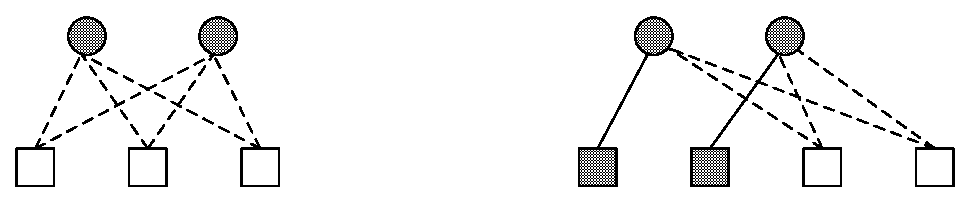
\includegraphics[width=3.45in,height=0.8in]{fig07.eps}
\caption{Candidate (2,b) absorbing sets}\label{Fig07}
\end{figure}
Suppose $a=2$. In $G_{p,3}$ an even number of edges from $D$
terminates in $\mathcal{E}(D)$. Thus either $b=0$ or $b=2$. These
correspond to the situations in Fig. \ref{Fig07}. In either case
there would be a cycle of length 4 in $G_{p,3}$, which is false
\cite{fan}. Thus $a\geq 3$.

Suppose $a=3$. In $G_{p,3}$ an even number of edges from $D$
terminates in $\mathcal{E}(D)$. Thus either $b=1$ or $b=3$.
Suppose $b=1$. This must correspond to the form in Fig.
\ref{Fig06},
\begin{figure}
\center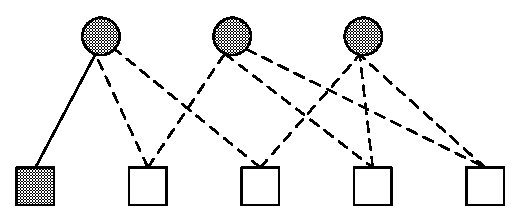
\includegraphics[width=1.9in,height=0.9in]{fig06a.eps}
\caption{Candidate (3,1) absorbing set}\label{Fig06}
\end{figure}
which implies the existence of a cycle of length 4 in $G_{p,3}$,
which is false \cite{fan}.

Thus $b=3$. Further, each bit node in $D$ would then connect to
exactly one check node in $\mathcal{O}(D)$ implying the unlabelled
form of Fig. \ref{Fig05a}.
%\begin{figure}
%\vspace{0.1in}\hspace{0.4in}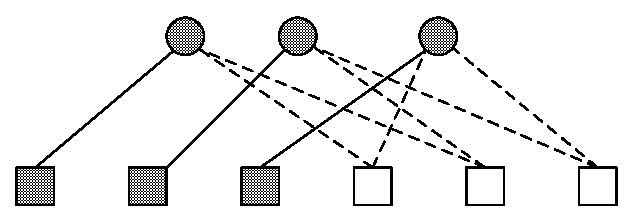
\includegraphics[width=2.5in,height=0.9in]{fig04.eps}
%\caption{Candidate (3,3) absorbing set}\label{Fig04}
%\end{figure}
Note that there is a cycle of length 6.

Suppose these $3$ bit nodes are indexed as $(j_1,k_1)$,
$(j_2,k_2)$ and $(j_3,k_3)$, respectively, where $j_1,j_2$ and
$j_3$ are distinct (by the edge consistency) and $0 \leq j_1, j_2,
j_3 \leq p-1$. Without loss of generality assume that $(j_1,k_1)$
and $(j_2,k_2)$ share a check in the row group $i_1$, $(j_2,k_2)$
and $(j_3,k_3)$ share a check in the row group $i_2$, and that
$(j_1,k_1)$ and $(j_3,k_3)$ share a check in the row group $i_3$,
where $i_1,i_2,i_3 \in \{0,1,2\}$ and are distinct by the vertex
consistency condition. This corresponds to the labelled
representation in Fig. \ref{Fig05a}.
%\begin{figure}
%\vspace{0.1in}\hspace{0.4in}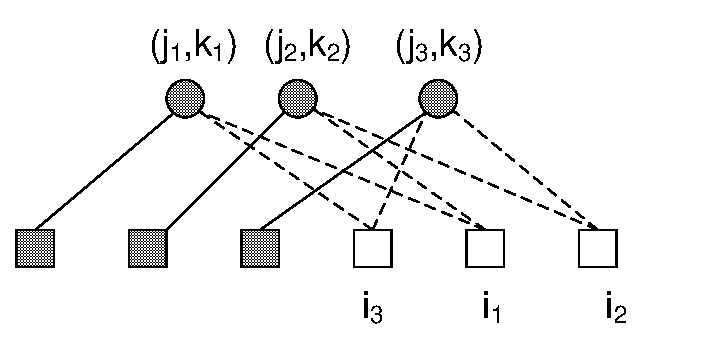
\includegraphics[width=2.7in,height=1.35in]{fig05a.ps}
%\caption{(Labelled) candidate (3,3) absorbing set}\label{Fig05}
%\end{figure}
\begin{figure}
\center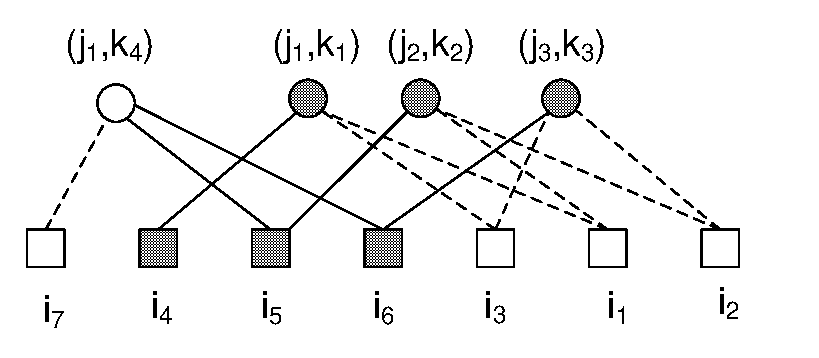
\includegraphics[width=2.7in,height=1.35in]{fig05c.eps}
\caption{Candidate (3,3) absorbing set (solid circles), with an
adjacent bit node (empty circle).}\label{Fig05a}
\end{figure}

Consider the matrix $M_1$ given by
\begin{equation}
M_1=(\sigma^{i_1j_1})^T(\sigma^{i_1j_2})(\sigma^{i_2j_2})^T(\sigma^{i_2j_3})(\sigma^{i_3j_3})^T(\sigma^{i_3j_1}).
\end{equation}
The matrix $M_1$ has a non-zero entry on the main diagonal, and
since it is itself a power of $\sigma$, it is necessary that
$M_1=\sigma^{p\ell}$, for some $\ell$, where $\ell$ is an integer.

It thus follows that\begin{equation}\label{eqpl}
p\ell=i_1(j_2-j_1)+i_2(j_3-j_2)+i_3(j_1-j_3).\end{equation}

By the symmetry of the absorbing set (see Fig. \ref{Fig05a}), we
may let $i_1=0$, $i_2=1$, and $i_3=2$. Since the column $k_1$ of
$\sigma^{2j_1}$ and column $k_3$ of $\sigma^{2j_3}$ have a
non-zero entry in the same row, it follows that
\begin{eqnarray}\label{eq12a}
k_1+2j_1 &\equiv & k_3+2j_3 \mod p.
\end{eqnarray}
Likewise,
\begin{eqnarray}\label{eq12b}
k_1 &\equiv& k_2   \mod p,\\
k_2 + j_2 &\equiv& k_3 +j_3  \mod p. \label{eq12c}
\end{eqnarray}
The existence of the solution for such a $(3,3)$ absorbing set is
given in Lemma~\ref{le11}. \comment{For example, a solution to
this constraint is for $\ell=0, i_1=0, i_2=2, i_3=1$ and $j_1=1$,
$j_2=(p-1)/2$, $j_3=p-2$. Since $(j_1,k_1)$ and $(j_2,k_2)$ share
a check in the row group $0$, it follows that $k_1=k_2$. Since the
column $k_1$ of $\sigma^{j_1}$ and column $k_3$ of $\sigma^{j_3}$
share a check in the row group 1, it follows that
\begin{eqnarray*}
k_1+j_1 &\equiv & k_3+j_3 \mod p.
\end{eqnarray*}

The indices of bit nodes participating in one such absorbing set
are $(k_1,j_1)$, $(k_1,j_2)$, and $([k_1-(p-3)]_p,j_3)$, for $k_1$
chosen arbitrary in the residue set$\mod p$.\hfill$\blacksquare$}

Even though the $(3,3)$ fully absorbing set seems plausible, care
must be taken with respect to a bit node \emph{outside} a
candidate fully absorbing set when this bit node also participates
in the unsatisfied checks. As we now show, such a $(3,3)$ fully
absorbing set cannot exist, though the existence of a $(3,3)$
absorbing set implies  a $(4,2)$ fully absorbing set.


Suppose first that a $(3,3)$ fully absorbing set exists. By
definition, it is then necessary that no bit node outside of the
absorbing set participates in more than one unsatisfied check
described by the absorbing set. Since $(j_1,k_1)$ and $(j_3,k_3)$
share a check, $j_1 \neq j_3$. Consider the bit node labelled
$(j_1,k_4)$ that connects to $i_6$, as in Figure \ref{Fig05a}.
Since $i_3=2$ and $i_2=1$, $i_6$ has value 0, and $k_3=k_4$. Note
that $i_5=2$ in Figure \ref{Fig05a}, since $i_1=0$, and $i_2=1$,
and by the vertex consistency condition at the bit node
$(j_3,k_3)$.

If the $(j_1,k_3)$ bit node does not also participate in the check
labelled with $i_5$ it would be necessary that $k_3+2j_1 \neq
k_2+2j_2 \mod p$, which is in contradiction with (\ref{eqpl})
through (\ref{eq12c}). Therefore the bit node $(j_1,k_3)$ shares
checks labelled with $i_5$ and $i_6$ with the bit nodes
$(j_2,k_2)$ and  $(j_3,k_3)$, respectively. This eliminates a
$(3,3)$ fully absorbing set for this configuration. This also now
implies a candidate $(4,2)$ fully absorbing set with bit nodes
$(j_1,k_1), (j_2,k_2)$, $(j_3,k_3)$ and $(j_1,k_3)$. Furthermore,
if a bit node labelled $(j_4,k_4)$ shares checks with the bit
nodes $(j_2,k_2)$ and $(j_,k_3)$ as above, $j_4=j_1$.

The cases where the bit node $(j_1,k_3)$ shares its remaining
check, which we label $i_7$, with one of $(j_1,k_1), (j_2,k_2)$,
or $(j_3,k_3)$ can be eliminated. By the vertex consistency
condition at the bit node $(j_1,k_3)$, $i_7=1$. By the girth
constraint, the bit node $(j_1,k_3)$ cannot share this check with
neither of $(j_2,k_2)$ and $(j_3,k_3)$. Since the bit node
$(j_1,k_1)$ already has the neighboring check whose label is
$i_4=1$, if the bit node $(j_1,k_3)$ also participates in this
check, it would imply the existence of a $(4,0)$ absorbing set,
which is impossible since the minimum distance of this code is 6,
\cite{helles}.

Therefore, in the resulting $(4,2)$ absorbing set, the unsatisfied
checks are labelled $i_4$ and $i_7$. Since $i_4=i_7=1$ no bit node
outside of this absorbing set can connect to both unsatisfied
checks, this $(4,2)$ configuration represents a fully absorbing
set.


It can be shown similarly that every $(4,2)$ fully absorbing set
has the shape as the unlabelled configuration in
Figure~\ref{Fig05a}, and that each can be obtained from an
underlying $(3,3)$ absorbing set. In particular, by the girth
condition, each unsatisfied check has degree 1 with respect to the
bits in the absorbing set (and these bits must be different by
definition of an absorbing set) and each neighboring satisfied
check has degree 2 with respect to the bits in the absorbing set.
To ensure that each bit node in the absorbing set has strictly
more satisfied than unsatisfied checks, it is further necessary
that the two bit nodes in the absorbing set with all neighboring
checks satisfied, each share a distinct check with one of the
remaining two bit nodes in the absorbing set, and one satisfied
check with each other. As a result, we arrive at the unlabelled
configuration in Figure~\ref{Fig05a}.


By symmetry, for each underlying $(3,3)$ absorbing set and for
each of the three choices of the labels of the resulting
unsatisfied check, there exists exactly one way of adjoining a
distinct fourth bit node that neighbors these unsatisfied checks.
Since the labels of the two unsatisfied checks are the same, each
resulting $(4,2)$ fully absorbing set comes from two different
$(3,3)$ underlying configurations.

 We complete the section with the following result.
\begin{lemma}\label{le11} The total number of $(3,3)$ absorbing sets and $(4,2)$ fully absorbing sets
in the Tanner graph described by $H_{p,3}$ is $p^2(p-1)$, and
$3p^2(p-1)/2$, respectively.
\end{lemma}
\noindent \textit{Proof:} It suffices to consider $\ell=-1,0,1$ in
(\ref{eqpl}).

For $\ell=0$, $2j_1=j_2+j_3$. For each value of $j_1$, $1 \leq j_1
\leq (p-1)/2$, there are $2j_1$ ways of assigning values to
$(j_1,j_2,j_3)$ (the cases where two of $j_1$,$j_2$ and $j_3$ are
the same have to be excluded by the edge consistency condition).
Likewise, for each $j_1$ where $(p+1)/2 \leq j_1 \leq p-2$ there
are $2(p-1-j_1)$ ways of assigning values to $(j_1,j_2,j_3)$. For
each assignment there are $p$ ways to assign values to
$(k_1,k_2,k_3)$ to ensure the validity of
(\ref{eq12a})-(\ref{eq12c}). In all, there is a total of
\[p\left[\sum_{j_1=1}^{(p-1)/2} 2j_1 + \sum_{j_1=(p+1)/2}^{p-2}
2(p-1-j_1)\right] = \frac{p(p-1)^2}{2}\] such assignments, each
describing a different $(3,3)$ absorbing set.

Likewise, for $\ell=1$ (and for $\ell=-1$ by symmetry) we require
$p+(j_2+j_3)=2j_1$. Thus $s=(j_2+j_3)$ is at most $p-2$ and odd.
For each such $s$, there are $s+1$ ways to assign the values to
$j_1,j_2$ and $j_3$, and for each such assignment, there are $p$
ways to assign values to $(k_1,k_2,k_3)$ to ensure the validity of
(\ref{eq12a})-(\ref{eq12c}). The total number of ways to select a
(3,3) absorbing set in this case is
\[
p\left[\sum_{s=1, s \text{
odd}}^{p-2}(s+1)\right]=\frac{p(p-1)(p+1)}{4}~.
\]

The total number of $(3,3)$ absorbing sets is thus $p^2(p-1)$.

Depending on which two of these three bit nodes the remaining bit
node $(j_4,k_4)$ (in the $(4,2)$ fully absorbing set) shares a
(satisfied) check with, we may assign $(j_4,k_4)$ in three
different ways. Note that in this way we have counted each $(4,2)$
set twice. Hence there are $3p^2(p-1)/2$ distinct $(4,2)$ fully
absorbing sets. \hfill$\blacksquare$


Since the codeword length $n$ is $p^2$, the result of Lemma
\ref{le11} implies Theorem~\ref{theo2} for $\gamma=3$. As a
comparison, the minimum distance of the $C_{p,\gamma}$ code is
$6$, \cite{helles}.
\subsection{Absorbing sets of
$H_{p,4}$}\label{theo14}


In order to establish that $(6,4)$ (fully) absorbing sets are
minimal for $H_{p,4}$, we will first show that $(a,b)$ absorbing
sets for $a < 6$ do not exist.

\comment{First, the condition $a<4$ is not possible as it would
violate the girth condition. For $a=4$, if $b<4$, there would
exist a bit node sharing at least two satisfied checks with some
other bit node in the absorbing set. If $b>4$, there would exist a
bit node in the absorbing set having more unsatisfied that
satisfied checks, which is not possible by definition. Thus, for
$a=4$, the only nontrivial candidate absorbing set is a $(4,4)$
absorbing set. }


Let $D$ denote an $(a,b)$ absorbing set in $G_{p,4}=(V,F,E)$, the
Tanner graph of $H_{p,4}$. If $a=2 (3)$ then at least $6 (9)$
edges from $D$ in $G_{p,4}$ terminate in $\mathcal{E}(D)$, which
implies the existence of a cycle of length 4 in $G_{p,4}$, which
is false \cite{fan}. Thus, $a \geq 4$.

Suppose $a=4$. The number of edges from $D$ in $G_{p,4}$ that
terminate in $\mathcal{E}(D)$ must be 12, 14, or 16, corresponding
to the cases $b$ = 4, 2, or 0, respectively. No check node in
$\mathcal{E}(D)$ can connect to all four of the bit nodes in $D$,
else there would need to be a cycle of length 4 in $G_{p,4}$,
which is false \cite{fan}. Thus, each check node in
$\mathcal{E}(D)$ connects to exactly two of the bit nodes in $D$.
There are $6$ pairs of nodes in $D$. Thus we must have $b=4$. The
following lemma establishes that such sets do not exist for large
enough prime $p$.


\begin{lemma}\label{Lem2} For $p>7$, the Tanner graph family $G_{p,4}$
does not contain any $(4,4)$ absorbing sets.
\end{lemma}
\noindent \textit{Proof:} No check node satisfied with respect to
the absorbing set has degree $> 2$, as otherwise there would exist
two bit nodes that share two distinct check nodes, which is not
possible by the girth condition \cite{fan}. Similarly, all bit
nodes in an absorbing set have distinct unsatisfied check nodes.

%\begin{figure}\hspace{1.0in}
%\begin{picture}(100,150)(0,0)
%\put(10,50){\line(1,0){60}} \put(10,110){\line(1,0){60}}
%\put(10,50){\line(0,1){60}} \put(70,50){\line(0,1){60}}
%\put(10,50){\line(1,1){60}} \put(10,110){\line(1,-1){60}}
%\put(0,40){{$(j_4,k_4)$}} \put(60,120){{$(j_2,k_2)$}}
%\put(0,120){{$(j_1,k_1)$}} \put(60,40){{$(j_3,k_3)$}}
%%\put(255,205){{$c_1^0(11)$='1'}}
%\put(0,80){{$i_4$}} \put(75,80){{$i_2$}} \put(40,120){{$i_1$}}
%\put(40,40){{$i_3$}} \put(31,90){{$i_5$}} \put(31,65){{$i_6$}}
%\end{picture}
%\caption{Depiction of the (4,4) set}
%\end{figure}
\begin{figure}
\center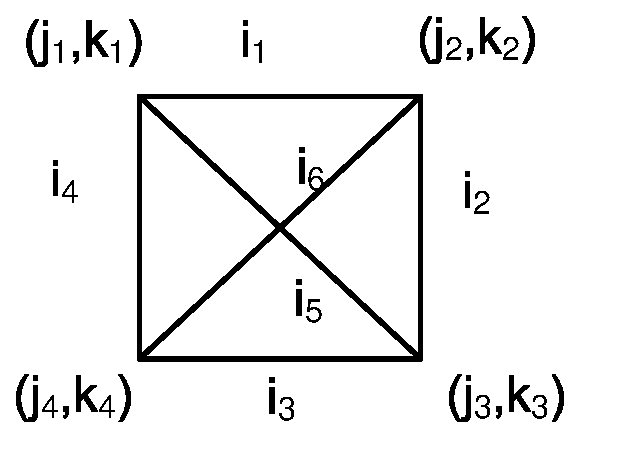
\includegraphics[width=2.65in,height=1.5in]{Drawing10_1.eps}
\caption{Depiction of the candidate (4,4) set} \label{fig44}
\end{figure}

Since each bit node in the absorbing set shares exactly 3
satisfied check nodes with other bit nodes in the absorbing set,
we can view the absorbing set as shown in Fig. \ref{fig44} where
each (labelled) vertex represents a distinct bit node and each
(labelled) edge represents a check node in which the bit nodes
associated with its endpoints participate.

By the edge consistency condition all $j_1$ through $j_4$ are
different. Since the column $k_1$ of $\sigma^{i_1j_1}$ and column
$k_2$ of $\sigma^{i_1j_2}$ have a non-zero entry in the same row,
it follows that
\begin{eqnarray*}
k_1+i_1j_1 &\equiv & k_2+i_1j_2 \mod p
\end{eqnarray*}

Likewise, for $i_2$ through $i_6$ we obtain
\begin{eqnarray*}
k_2+i_2j_2 &\equiv& k_3+i_2j_3 \mod p, \\
k_3+i_3j_3 &\equiv& k_4+i_3j_4 \mod p, \\
k_1+i_4j_1 &\equiv& k_4+i_4j_4 \mod p, \\
k_1+i_5j_1 &\equiv& k_3+i_5j_3 \mod p, \text{and}\\
k_2+i_6j_2 &\equiv& k_4+i_6j_4 \mod p.
\end{eqnarray*}

Moreover, by imposing the vertex consistency condition and
exploiting the symmetry, it suffices to consider
$(i_1,i_2,i_3,i_4,i_5,i_6)$ either $(x,y,x,y,z,z)$ or
$(x,y,x,y,z,w)$ where $x,y,z,w \in \{0,1,2,3 \}$ and are distinct.

For the case $(x,y,x,y,z,z)$, we establish the following
conditions based on the cycles within the graph in Fig.
\ref{fig44}:
\begin{eqnarray*}
p\ell_1&=&x(j_2-j_1)+y(j_3-j_2)+z(j_1-j_3), \\
p\ell_2&=&x(j_2-j_1)+z(j_4-j_2)+y(j_1-j_4),\text{and}\\
p\ell_3&=&x(j_4-j_3)+y(j_1-j_4)+z(j_3-j_1).
\end{eqnarray*}
for some integers $\ell_1,\ell_2$ and $\ell_3$.

From this system it follows that
\begin{eqnarray*}
p\ell_1'&=&(y-z)(j_3+j_4-j_1-j_2),\\
p\ell_2'&=&(x-z)(j_2+j_3-j_1-j_4),\text{and}\\
p\ell_3'&=&(x-y)(j_2+j_4-j_1-j_3).
\end{eqnarray*}

\noindent for some integers $\ell_1',\ell_2'$ and $\ell_3'$. Since
$x,y,z$ are distinct, all $j$'s would have to be the same, which
contradicts the edge consistency constraint.

For the case $(x,y,x,y,z,w)$ we have that
\begin{eqnarray*}
p\ell_1&=&x(j_2-j_1)+y(j_3-j_2)+z(j_1-j_3),\\
p\ell_2&=&x(j_2-j_1)+w(j_4-j_2)+y(j_1-j_4), \text{and}\\
p\ell_3&=&x(j_4-j_3)+y(j_1-j_4)+z(j_3-j_1).
\end{eqnarray*}
for some integers $\ell_1,\ell_2$ and $\ell_3$.

By manipulating above conditions one arrives at
\begin{equation}\label{eq23}
(z-x)(w-y)+(z-y)(w-x) \equiv 0 \mod p.
\end{equation}

It can be easily verified that this condition can not hold for any
choice of $x,y,z,w$, where $x,y,z,w \in \{0,1,2,3 \}$ and are
distinct for $p>7$. \hfill$\blacksquare$

We next show that $(5,b)$ absorbing sets do not exist.
\begin{lemma}\label{Lem3} For $p>19$, the Tanner graph family $G_{p,4}$
does not contain any $(5,b)$ absorbing sets.
 \end{lemma}

\noindent \textit{Proof:} Since each bit node in the absorbing set
has at most one neighboring unsatisfied check node, it follows
that $b \leq 5$. Observe that the number of bit nodes with 3
satisfied and 1 unsatisfied check nodes is even, and thus $b$ is
even. First $b>0$ by the minimum distance, $d_{min}\geq 8$
\cite{helles} of the code. If $b=2$ and all satisfied check nodes
had degree 2, such an absorbing set would contain a $(4,4)$
absorbing set, which by Lemma \ref{Lem2} does not exist. A
degree-4 satisfied check node would violate the girth condition.


We are thus left with analyzing $b=4$ with all satisfied check
nodes of degree 2. Note that by the girth condition, all
unsatisfied checks have degree 1 with respect to the bits in the
absorbing set. Therefore, this candidate absorbing sets contains 1
bit node with all checks satisfied and 3 bit nodes each with 3
satisfied and 1 unsatisfied check. The only way that such an
absorbing set could exist is if one has the configuration shown in
Fig. \ref{fig52}, where the vertices represent bit nodes and edges
represent their satisfied check nodes.
%we have that $i_1$ connect $(k_1,j_1)$ and
%$(k_2,j_2)$, $i_2$ connect $(k_1,j_1)$ and $(k_3,j_3)$, $i_3$
%connect $(k_1,j_1)$ and $(k_4,j_4)$, $i_4$ connect $(k_1,j_1)$ and
%$(k_5,j_5)$, $i_5$ connect $(k_2,j_2)$ and $(k_3,j_3)$, $i_6$
%connect $(k_2,j_2)$ and $(k_4,j_4)$, $i_7$ connect $(k_3,j_3)$ and
%$(k_5,j_5)$, and $i_8$ connect $(k_4,j_4)$ and $(k_5,j_5)$, as

%\begin{figure}\hspace{1.0in}
%\begin{picture}(100,150)(0,0)
%\put(10,50){\line(1,0){60}} \put(10,110){\line(1,0){60}}
%\put(10,50){\line(0,1){60}} \put(70,50){\line(0,1){60}}
%\put(10,50){\line(1,1){60}} \put(10,110){\line(1,-1){60}}
%\put(0,40){{$(j_4,k_4)$}} \put(60,120){{$(j_2,k_2)$}}
%\put(0,120){{$(j_1,k_1)$}} \put(60,40){{$(j_3,k_3)$}}
%%\put(255,205){{$c_1^0(11)$='1'}}
%\put(0,80){{$i_4$}} \put(75,80){{$i_2$}} \put(40,120){{$i_1$}}
%\put(40,40){{$i_3$}} \put(31,90){{$i_5$}} \put(31,65){{$i_6$}}
%\end{picture}
%\caption{Depiction of the candidate (5,2) set}
%\end{figure}

\begin{figure}
\center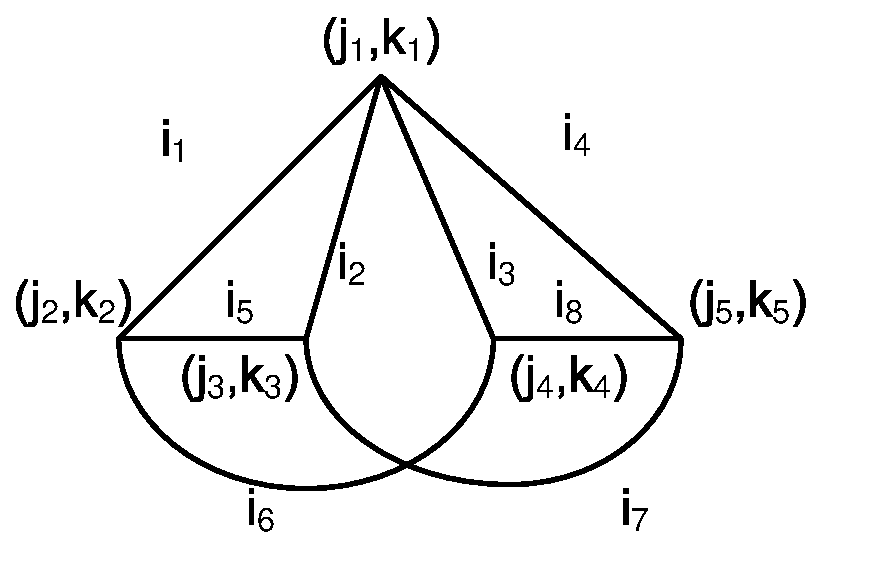
\includegraphics[width=3.0in,height=1.8in]{Drawing22_1.eps}
\caption{Depiction of the candidate (5,4) set} \label{fig52}
\end{figure}

Since $i_1$, $i_2$, $i_3$ and $i_4$ are all distinct by the vertex
consistency condition, we may assume that $i_1=0$. Then moreover,
either $i_7=0$ or $i_8=0$ by the vertex consistency at $(j_5,k_5)$
and $(j_4,k_4)$.

If $i_7=0$ we let $x=i_2=i_8$, $y=i_3=i_5$ and $z=i_4=i_6$ (by the
vertex consistency condition) where $x,y,z \in \{1,2,3\}$ and are
distinct. Note that $k_1=k_2$ and $k_3=k_5$. We also obtain
\begin{eqnarray*}
k_1+xj_1 &\equiv& k_3+xj_3 \mod p, \\
k_1+yj_1 &\equiv& k_4+yj_4 \mod p, \\
k_1+zj_1 &\equiv& k_5+zj_5 \mod p, \\
k_2+yj_2 &\equiv& k_3+yj_3 \mod p, \\
k_2+zj_2 &\equiv& k_4+zj_4 \mod p, \text{and}\\
k_4+xj_4 &\equiv& k_5+xj_5 \mod p.
\end{eqnarray*}

and likewise for $i_8=0$ we let $x=i_2=i_6$, $y=i_3=i_7$ and
$z=i_4=i_5$. Note that now $k_1=k_2$ and $k_4=k_5$ and
\begin{eqnarray*}
k_1+xj_1 &\equiv& k_3+xj_3 \mod p, \\
k_1+yj_1 &\equiv& k_4+yj_4 \mod p, \\
k_1+zj_1 &\equiv& k_5+zj_5 \mod p, \\
k_2+zj_2 &\equiv& k_3+zj_3 \mod p, \\
k_2+xj_2 &\equiv& k_4+xj_4 \mod p, \text{and}\\
k_3+yj_3 &\equiv& k_5+yj_5 \mod p.
\end{eqnarray*}

where $x,y,z\in \{1,2,3\}$ and distinct.

In the first case, let $a=j_3-j_1$, $b=j4-j_1$, $c=j_5-j_1$, and
$d=j_3-j_2$. Note that by the consistency conditions, not all $a$,
$b$, $c$, $d$ can be zero. We then obtain

\begin{equation}
\left[\begin{array}{ccccc}
x & 0 & -z & 0\\
x & 0 & 0 & -y\\
z & y-z&0 & -z\\
x & x-y & -x & 0
\end{array}
\right] \left[\begin{array}{c}a\\b\\c\\d\end{array} \right] =
\left[\begin{array}{c}0\\0\\0\\0\end{array} \right].
\end{equation}

As a result,
\begin{equation}\label{eq5a}
xy(z-x)(z-y)-z^2(x-y)^2 \equiv 0 \mod p~.
\end{equation}

In the second case, we likewise let $a=j_3-j_1$, $b=j4-j_1$,
$c=j_5-j_1$, and $d=j_3-j_2$. Note that by the consistency
conditions, not all $a$, $b$, $c$, $d$ can be zero. We then obtain

\begin{equation}
\left[\begin{array}{ccccc}
0 & y & -z & 0\\
x & y-x & 0 & -x\\
z & 0 &0 & -z\\
y-x & y & -y & 0
\end{array}
\right] \left[\begin{array}{c}a\\b\\c\\d\end{array} \right] =
\left[\begin{array}{c}0\\0\\0\\0\end{array} \right]~,
\end{equation}
from which the constraint~\ref{eq5a} also follows.


Since the constraint ~\ref{eq5a} does not have a solution for $p>19$
for distinct $x,y,z \in
\{1,2,3\}$, the proof of the Lemma follows.\hfill$\blacksquare$ %\footnote{As a side remark, we note that equation
%(\ref{eq5a}) does have a solution for $p \in \{5,11,19$\}.}

%No 4 deg. checks. dmin is 8.
%\begin{remark}

We can now proceed with the analysis of $(6,b)$ absorbing sets.
Since the number of bit nodes with 3 satisfied and 1 unsatisfied
check node is even, $b$ is even. First, $b=0$ is not possible
since $d_{min} \geq 8$ \cite{helles}. The following lemma
considers $b=2$.

\comment{ Observe that there cannot be a check of degree 4 with
respect to the bits in a $(6,b)$ absorbing set, as otherwise the
girth condition would be violated. As a result, in the remainder
of the analysis we will assume that all checks that have even
number of bit node neighbors in a $(6,b)$ absorbing set have
degree 2 with respect to the absorbing set. Moreover, since
$d_{min} \geq 8$ \cite{helles} and since all bit nodes in the
$(6,b)$ absorbing set have at most one unsatisfied check (with
respect to the absorbing set), it suffices to consider $b$ even
and positive.}
%\end{remark}

\comment{ Observe that there cannot be a check of degree 4 with
respect to the bits in a $(6,b)$ absorbing set, as otherwise the
girth condition would be violated. As a result, in the remainder
of the analysis we will assume that all checks that have even
number of bit node neighbors in a $(6,b)$ absorbing set have
degree 2 with respect to the absorbing set. Moreover, since
$d_{min} \geq 8$ \cite{helles} and since all bit nodes in the
$(6,b)$ absorbing set have at most one unsatisfied check (with
respect to the absorbing set), it suffices to consider $b$ even
and positive.}
%\end{remark}

\begin{lemma}\label{Lem4} For $p>19$, the Tanner graph family $G_{p,4}$ does not contain any $(6,2)$ absorbing sets.
\end{lemma}

\noindent \textit{Proof:}
%\begin{figure}\hspace{1.0in}
%\begin{picture}(100,150)(0,0)
%\put(10,50){\line(1,0){60}} \put(10,110){\line(1,0){60}}
%\put(10,50){\line(0,1){60}} \put(70,50){\line(0,1){60}}
%\put(10,50){\line(1,1){60}} \put(10,110){\line(1,-1){60}}
%\put(0,40){{$(j_4,k_4)$}} \put(60,120){{$(j_2,k_2)$}}
%\put(0,120){{$(j_1,k_1)$}} \put(60,40){{$(j_3,k_3)$}}
%%\put(255,205){{$c_1^0(11)$='1'}}
%\put(0,80){{$i_4$}} \put(75,80){{$i_2$}} \put(40,120){{$i_1$}}
%\put(40,40){{$i_3$}} \put(31,90){{$i_5$}} \put(31,65){{$i_6$}}
%\end{picture}
%\begin{picture}(100,150)(0,0)
%\put(10,50){\line(1,0){60}} \put(10,110){\line(1,0){60}}
%\put(10,50){\line(0,1){60}} \put(70,50){\line(0,1){60}}
%\put(10,50){\line(1,1){60}} \put(10,110){\line(1,-1){60}}
%\put(0,40){{$(j_4,k_4)$}} \put(60,120){{$(j_2,k_2)$}}
%\put(0,120){{$(j_1,k_1)$}} \put(60,40){{$(j_3,k_3)$}}
%%\put(255,205){{$c_1^0(11)$='1'}}
%\put(0,80){{$i_4$}} \put(75,80){{$i_2$}} \put(40,120){{$i_1$}}
%\put(40,40){{$i_3$}} \put(31,90){{$i_5$}} \put(31,65){{$i_6$}}
%\end{picture}
%\caption{Depiction of the candidate (6,2) sets}
%\end{figure}
\begin{figure}
\center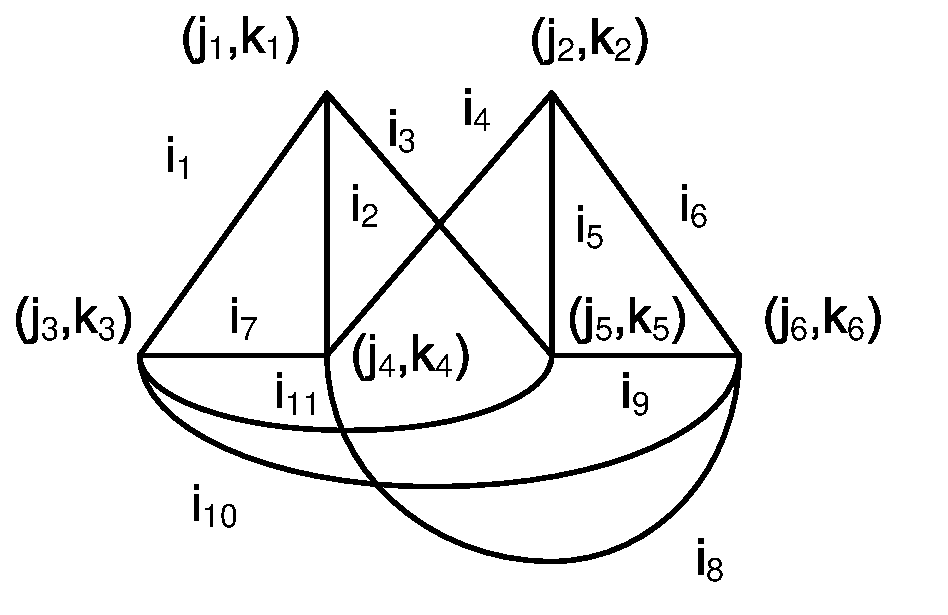
\includegraphics[width=3.5in,height=2.2in]{Drawing30_2.eps}
\newline
\center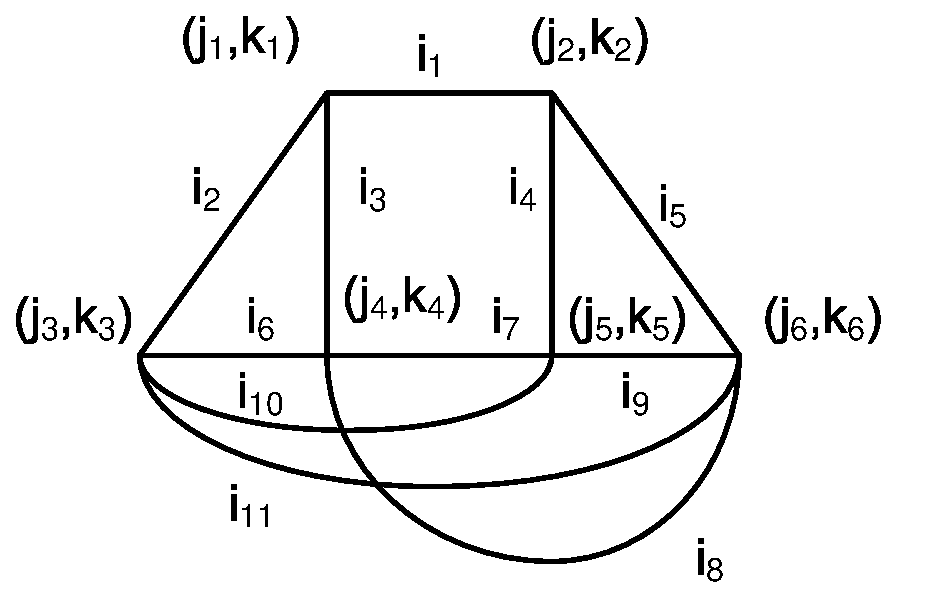
\includegraphics[width=3.5in,height=2.2in]{Drawing32_1.eps}\hspace{0.3in}
\caption{Depiction of the candidate (6,2) sets} \label{fig62}
\end{figure}
We first show that there is no check node of degree at least 4
with respect to the bit nodes in the absorbing set. If this were
possible, there would exist at least 2 bit nodes  in the absorbing
set with all check nodes satisfied and with a shared check node of
degree at least 4. They would necessarily share another check
node, which is not possible by the girth condition \cite{fan}.

We can now focus on the case where all satisfied check nodes with
respect to the absorbing set have degree 2. By requiring that each
vertex corresponding to a bit node in the absorbing set has either
3 or 4 outgoing edges, and that there are no parallel edges, it
follows that there are 2 possible configurations, as shown in
Figure \ref{fig62}, that relate bit nodes in the absorbing set
(vertices) and their shared satisfied checks (edges). Note that it
is apriori possible to have an unsatisfied check of degree 3 with
respect to the bit nodes in the absorbing set. This condition is
not a part of Figure\ref{fig62}.

Observe that the bottom configuration contains a $(4,4)$ absorbing
set which consists of $(j_3,k_3)$, $(j_4,k_4)$, $(j_5,k_5)$, and
$(j_6,k_6)$. By Lemma \ref{Lem2} such configuration is not
possible for $p>7$.

 By ensuring vertex consistency, it follows that the top
configuration in Figure 3 has 2 distinct edge labellings.
Specifically, using the vertex consistency condition, we have for
the top configuration
\begin{eqnarray*}
k_1+i_1j_1 &\equiv& k_3+i_1j_3 \mod p, \\
k_1+i_2j_1 &\equiv& k_4+i_2j_4 \mod p, \\
k_1+i_3j_1 &\equiv& k_5+i_3j_5 \mod p, \\
k_2+i_4j_2 &\equiv& k_4+i_4j_4 \mod p, \\
k_2+i_5j_2 &\equiv& k_5+i_5j_5 \mod p, \\
k_2+i_6j_2 &\equiv& k_6+i_6j_6 \mod p, \\
k_3+i_7j_3 &\equiv& k_4+i_7j_4 \mod p, \\
k_4+i_8j_4 &\equiv& k_6+i_8j_6 \mod p, \\
k_5+i_9j_5 &\equiv& k_6+i_9j_6 \mod p, \\
k_3+i_{10}j_3 &\equiv& k_6+i_{10}j_6 \mod p,\text{and} \\
k_3+i_{11}j_3 &\equiv& k_5+i_{11}j_5 \mod p,
\end{eqnarray*}
and either \[x=i_1=i_5=i_8, y=i_7=i_9, z=i_2=i_6=i_{11},
w=i_3=i_4=i_{10} \hspace{0.2in}(\star) \text{ or }\]
\[x=i_1=i_4=i_9, y=i_3=i_6=i_7, z=i_8=i_{11}, w=i_2=i_5=i_{10}
\hspace{0.2in}(\star\star)\] where throughout $x,y,z,w$ are distinct
and belong to the set $\{0,1,2,3\}$.

We will now show that in each case we arrive at one of the following
constraints:
\begin{equation}\label{consti}
\begin{array}{ccccc}
\tilde{x} &\equiv& \tilde{y} &\mod p, &\text{or} \\
\tilde{x}\tilde{z}(\tilde{z}-\tilde{y})(\tilde{x}-\tilde{y})
&\equiv& \pm \tilde{y}^2(\tilde{x}-\tilde{z})^2  &\mod p, &{}
\end{array}
\end{equation}

where $\{\tilde{x},\tilde{y},\tilde{z}\} = \{x,y,z\}= \{1,2,3\}$ and
are distinct.

Note that exactly one of $x,y,z,w$ has value $0$, and the remainder
three constitute the set $\{1,2,3\}$.

For the first case ($\star$) we separately consider $x=0$, $y=0$,
$z=0$, and $w=0$.

1. For $x=0$ we obtain \begin{equation}\begin{array}{ccccc} k_1-k_4
&\equiv z(j_4-j_1)& \equiv y(j_4-j_3)& \equiv w(j_6-j_3) &\mod p
\\
k_2-k_4 &\equiv w(j_4-j_2) &\equiv  z(j_6-j_2) &\equiv y(j_6-j_5)
&\mod
p\\
k_1-k_2 &\equiv w(j_5-j_1) &\equiv z(j_5-j_3) & {}&\mod p~.
\end{array}\end{equation}

Since $\{y,z,w\}=\{1,2,3\}$ by construction, they share no common
nontrivial factors, and we may let
\begin{equation}\begin{array}{ccccc}k_1-k_4 &\equiv& ywzt &\mod p, &{} \\
k_2-k_4 &\equiv& ywzu &\mod p, &\text{ and }\\k_1-k_2 &\equiv& wzs
&\mod p&{}
\end{array}\end{equation}

for some integers $t,s$ and $u$ which are themselves nonzero by
construction. Some algebra yields
\begin{equation}\begin{array}{cccc}
s &\equiv &yt-yu &\mod p \\
ws &\equiv &-wzu +yzt &\mod p\\
zs &\equiv &-wzu +ywu -yzu +ywt &\mod p~.
\end{array}\end{equation}


The last set of constraints implies $w\equiv z \mod p$ which is in
contradiction with initial constraints. Note that this is precisely
the first condition in \eqref{consti} with the substitution
$w=\tilde{x}$ and $z=\tilde{y}$.

2. For $y=0$ we obtain \begin{equation}\begin{array}{cccccc} k_1-k_3
&\equiv x(j_3-j_1)& \equiv z(j_4-j_1)& {} &\mod p
\\
k_2-k_5 &\equiv x(j_5-j_2) &\equiv  z(j_6-j_2) &{} &\mod
p\\
k_3-k_5 &\equiv x(j_6-j_4) &\equiv w(j_6-j_3) &
\equiv z(j_5-j_3)&\mod p\\
k_1-k_5 &\equiv w(j_5-j_1) & {} & {} &\mod p~.
\end{array}\end{equation}

Since $\{x,z,w\}=\{1,2,3\}$, we may let
\begin{equation}\begin{array}{ccccc}k_1-k_3 &\equiv& xzs &\mod p, &{} \\
k_1-k_5 &\equiv & wv &\mod p, &{}\\ k_2-k_5 &\equiv& xzu &\mod p,
&\text{ and }\\k_3-k_5 &\equiv& xwzt &\mod p&{}
\end{array}\end{equation}

for some integers $s,u,v$ and $t$, which are themselves nonzero by
construction. Some algebra yields
\begin{equation}\begin{array}{cccc}
xzs &\equiv &wv-xwzt &\mod p \\
v &\equiv &xwt+zs &\mod p \\
xs & \equiv& -wzt +xzt+zs &\mod p~,
\end{array}\end{equation}
from which it follows that
\begin{equation}
z^2(x-w)^2 \equiv xw(w-z)(x-z) \mod p~.
\end{equation}
Note that this is precisely the second condition in \eqref{consti}
with substitution $x=\tilde{x}$, $z=\tilde{y}$, and $w=\tilde{z}$
and the plus sign on the right side of \eqref{consti}.

3. For $z=0$ we obtain
\begin{equation}\begin{array}{ccccc} k_1-k_3
&\equiv x(j_3-j_1)& \equiv w(j_5-j_1)& \equiv y(j_3-j_4) &\mod p
\\
k_2-k_3 &\equiv x(j_5-j_2) &\equiv  y(j_5-j_6) &\equiv w(j_3-j_6)
&\mod
p\\
k_1-k_2 &\equiv w(j_2-j_4) &\equiv x(j_6-j_4) & {}&\mod p~.
\end{array}\end{equation}


As before, some algebra yields $x\equiv w \mod p$, which with the
substitution $x=\tilde{x}$, $y=\tilde{y}$ corresponds to the first
condition in \eqref{consti}.

 4. For $w=0$ we obtain
\begin{equation}\begin{array}{ccccc} k_1-k_3
&\equiv x(j_3-j_1)& \equiv y(j_6-j_5)& \equiv z(j_3-j_5) &\mod p
\\
k_2-k_3 &\equiv z(j_6-j_2) &\equiv  y(j_3-j_4) &\equiv x(j_6-j_4)
&\mod
p\\
k_1-k_2 &\equiv z(j_4-j_1) &\equiv x(j_2-j_5) & {}&\mod p~.
\end{array}\end{equation}

After some manipulation, we obtain the following condition
\begin{equation}
xz(z-y)(x-y) \equiv -y^2(x-z)^2 \mod p,
\end{equation}
which can be seen to correspond to the second condition in
\eqref{consti} with the minus sign on the right hand side and the
substitution $x=\tilde{x}$, $y=\tilde{y}$, and $z=\tilde{z}$.

For the second case ($\star \star $) we separately consider $x=0$,
$y=0$, $z=0$, and $w=0$, and proceed along the lines of the previous
case to arrive at the desired conditions \eqref{consti}.

For $x=0$, resp. $y=0$, it follows after some algebra that $y \equiv
w \mod p$, resp. $x \equiv w \mod p$, which is precisely the first
condition in \eqref{consti} with the substitution $y=\tilde{x}$ and
$w=\tilde{y}$, resp. $x=\tilde{x}$ and $w=\tilde{y}$.


For $z=0$, resp. $w=0$, it follows similarly that $xw(w-y)(x-y)
\equiv y^2(x-w)^2 \mod p$, resp. $xy(y-z)(x-z) \equiv -z^2(x-y)^2
\mod p$, both of which correspond to the second condition in
\eqref{consti} with appropriate substitutions.


It can be verified that the conditions stated in \eqref{consti}
cannot hold for $p>19$, which completes the proof of the Lemma.
\hfill$\blacksquare$

Having eliminated smaller candidate absorbing sets, we now prove the
following result.

\begin{lemma}\label{Lem5} For all $p > 5$, the Tanner graph family $G_{p,4}$ has $(6,4)$ (fully) absorbing
sets.
\end{lemma}

\noindent \textit{Proof:}
\begin{figure}[ht]
\center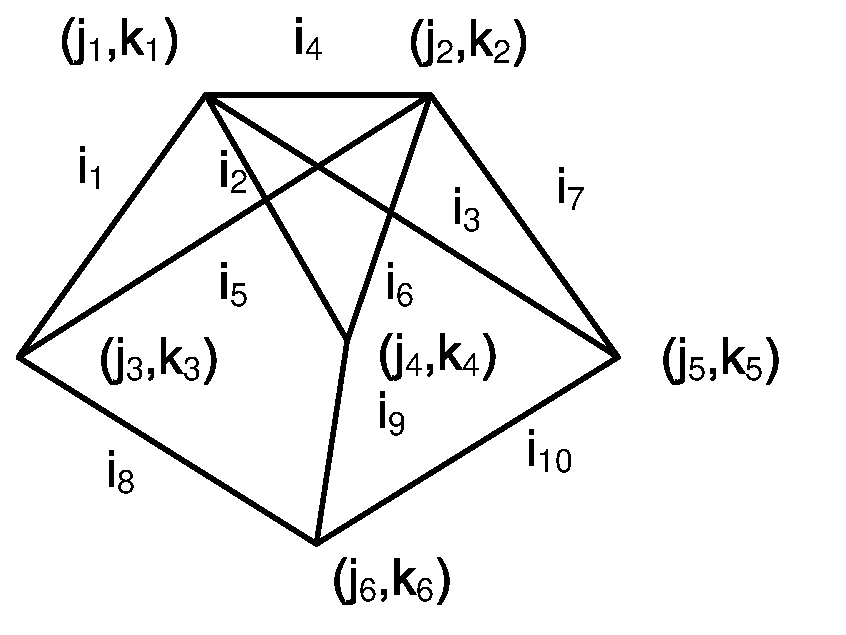
\includegraphics[width=3.5in,height=2.5in]{Drawing641_1.eps}
\caption{Depiction of the first candidate (6,4) set} \label{fig64a}
\end{figure}
\begin{figure}[ht]
\center
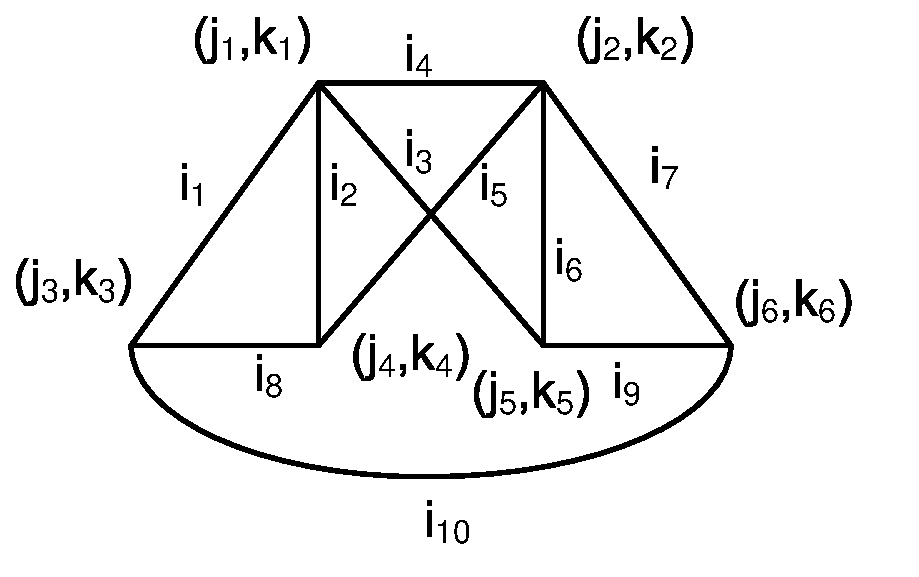
\includegraphics[width=3.5in,height=2.3in]{Drawing642_2.eps}
\caption{Depiction of the second candidate (6,4) set} \label{fig64b}
\end{figure}
\begin{figure}[ht]
\center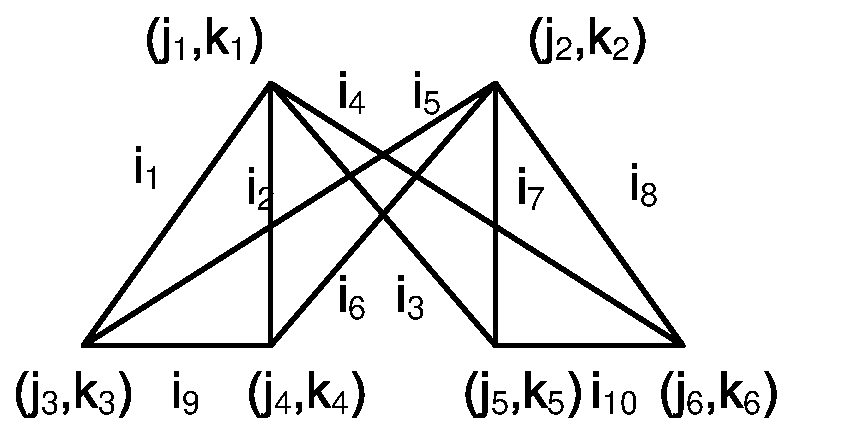
\includegraphics[width=3.5in,height=1.8in]{Drawing643_1.eps}
\caption{Depiction of the third candidate (6,4) set} \label{fig64c}
\end{figure}
First note that there cannot be a degree-6 check with respect to
the bits in the absorbing set as then some of these bits would
have to share another satisfied check which is not possible by the
girth condition. Suppose that there exists a check node of degree
4 with respect to a $(6,4)$ absorbing set. Let $t_1, t_2,t_3,t_4$
be the bit nodes in the absorbing set participating in degree-4
check node, and let $t_5$ and $t_6$ be the remaining two bit nodes
in the absorbing set. By the girth condition there can be at most
one degree-4 check incident to the bit nodes in the absorbing set.
If at least one of $t_1, t_2,t_3,t_4$ had all check nodes
satisfied, it would be necessary that such a bit node shares
another distinct check node with some other bit node participating
in the degree-4 check node, which is impossible by the girth
constraint \cite{fan}. Thus, all of $t_1, t_2,t_3,t_4$ are each
connected to 3 satisfied and 1 unsatisfied check node. Then $t_5$
and $t_6$ are each connected to 4 satisfied check nodes each of
degree 2 with respect to the bit nodes in the absorbing set. Since
$t_1$ through $t_4$ have 3 satisfied neighboring checks (one of
which is a degree-4 check by assumption), they each share a check
with $t_5$ and with $t_6$. Therefore, $t_5$ and $t_6$ do not share
a check. Let $i_j$ for $1 \leq j \leq 4$ be the labels of the
three check nodes connecting $t_j$ and $t_5$. By the vertex
consistency condition at $t_5$, they are all different. By the
vertex consistency condition at each of $t_j$ for $1 \leq j \leq
4$ the label of their shared degree-4 check node must be different
from all $i_j$ for $1 \leq j \leq 4$, which is impossible as there
are only 4 distinct labels available. Therefore all satisfied
check nodes neighboring bit nodes in the absorbing set have degree
2.



One can show that there are 3 possible non isomorphic
configurations, as shown in Figure~\ref{fig64a},~\ref{fig64b},
and~\ref{fig64c}. By ensuring the vertex consistency, it further
follows that for each configuration there are 8 distinct edge
labellings.

Let us consider the topmost configuration first. The other two
configurations are analyzed similarly subsequently.

I. \underline{Candidate (6,4) configuration, given in Figure
~\ref{fig64a}.}

As before, we establish a congruential constraint for each triplet
consisting of an edge and its endpoints given in the topmost
Figure~\ref{fig64a}. The set of constraints consisting of 10 such
equations, one for each edge, is
\begin{eqnarray*}
k_1+i_1j_1 &\equiv& k_3+i_1j_3 \mod p, \\
k_1+i_2j_1 &\equiv& k_4+i_2j_4 \mod p,\\
k_1+i_3j_1 &\equiv& k_5+i_3j_5 \mod p, \\
k_1+i_4j_1 &\equiv& k_2+i_4j_2 \mod p, \\
k_2+i_5j_2 &\equiv& k_3+i_5j_3 \mod p, \\
k_2+i_6j_2 &\equiv& k_4+i_6j_4 \mod p, \\
k_2+i_7j_2 &\equiv& k_5+i_7j_5 \mod p, \\
k_3+i_8j_3 &\equiv& k_6+i_8j_6 \mod p, \\
k_4+i_9j_4 &\equiv& k_6+i_9j_6 \mod p,\text{and} \\
k_5+i_{10}j_5 &\equiv& k_6+i_{10}j_6 \mod p.
\end{eqnarray*}
We now determine all possible edge labellings. For convenience, we
assign $(i_1,i_2,i_3,i_4)$ $\asn$ $(x,y,z,w)$, where $x,y,z,w \in
\{0,1,2,3 \}$ and distinct. Then, by imposing the vertex consistency
conditions, the assignments for the remaining edge labels are as
follows
\begin{eqnarray*}\label{tuples} (i_5,i_6,i_7,i_8,i_9,i_{10}) \in
 \{(y,z,x,z,x,y), (z,x,y,y,z,x),  \\ (y,z,x,z,w,y),
(y,z,x,w,x,y),  (y,z,x,z,x,w),\\(z,x,y,y,z,w)
(z,x,y,y,w,x),(z,x,y,w,z,x) \}.
\end{eqnarray*}

We first observe that the assignments
$(i_1,i_2,i_3,i_4,i_5,i_6,i_7,i_8,i_9,i_{10})=(x,y,z,w,y,z,x,z,x,y)$
and
$(i_1,i_2,i_3,i_4,i_5,i_6,i_7,i_8,i_9,i_{10})=(x,y,z,w,z,x,y,y,z,x)$
are in fact symmetric and is thus sufficient to analyze only one of
them.

Likewise, by appealing to symmetry and after appropriate
renamings, the remaining six assignments also represent the same
labelled configuration.

 Consider the tuple
$(i_1,i_2,i_3,i_4,i_5,i_6,i_7,i_8,i_9,i_{10})$=
$(x,y,z,w,y,z,x,z,x,y)$. By symmetry of the configuration it is
sufficient to consider $x=0$ and $w=0$. Specifically, letting $y=0$
or $z=0$ reduces to the $x=0$ case.

For $x=0$ we then obtain
\begin{equation}\begin{array}{ccccc}
k_1-k_4 &\equiv y(j_4-j_1) &\equiv z(j_6-j_3) &{}& \mod p\\
k_2-k_4 &\equiv z(j_4-j_2) & \equiv y(j_6-j_5) &{} & \mod p\\
 k_1-k_2 &\equiv z(j_5-j_1) & \equiv w(j_2-j_1) &\equiv y(j_2-j_3)& \mod p~.
\end{array}\end{equation}


For convenience we let
\begin{equation}\begin{array}{cccc}
k_1-k_4 &\equiv yzv &\mod p \\
k_1-k_2 &\equiv yzwt &\mod p\\
k_2-k_4 &\equiv yzs &\mod p,
\end{array}\end{equation}
for appropriately chosen integers $v,t$ and $s$.

By fixing the values of $j_1$ and $t$, the rest of $j_2$ through
$j_6$ as well as $u$ and $s$ follow uniquely for chosen $y,z$ and
$w$ since based on the above we may write
\begin{equation}
\left[ \begin{array}{ccccccc} 0 & 0 & 1 & 0 & 0 & -z &0\\
0 & 0 & 0 & 1 & 0 & 0 &0\\
1 & 0 & 0 & 0 & 0 & 0 &0\\
1 & -1 & 0 & 0 & 0 & 0 &0\\
-1 & 0 & 1 & 0 & 0 & 0 &-y\\
0 & -1 & 0 & 0 & 1 & -y &0\\
0 & 0 & 0 & -1 & 1 & 0 & -z
\end{array}\right] \left[\begin{array}{c}
j_2\\j_3\\j_4\\j_5\\j_6\\v\\s\end{array}\right] \equiv
\left[\begin{array}{c}j_1\\j_1+ywt\\j_1+yzt\\zwt\\0\\0\\0\end{array}\right]
\mod p~.
\end{equation}

Note that neither the vector multiplying the matrix nor the vector
on the right hand side cannot be an all-zeros vector as otherwise
the consistency conditions would be violated.

By inverting the matrix above, and using the relationships of these
variables with $k_1$ through $k_6$ we obtain the system of solutions
listed in Figure~\ref{table64}. As indicated, each row in the table
corresponds to a different numerical assignment of $y$, $z$ and $w$.
In the table $q$, $t$ and $s$ are arbitrary residues $\mod p$ and
the entries should be interpreted $\mod p$. Note that we have thus
established the existence of $(6,4)$ absorbing sets.

Furthermore, under the current configuration, the bit nodes in one
such $(6,4)$ absorbing set that have 3 satisfied and 1 unsatisfied
check, all have unsatisfied checks in the row group labelled $w$. By
the edge consistency condition, no bit node can connect to more than
one such check. Therefore, this configuration is in fact a $(6,4)$
fully absorbing set.

The (absolute) indices of columns that correspond to the bit nodes
in the absorbing set are $k_i+pj_i$ for $1 \leq i \leq 6$ and the
indices of rows that correspond to the unsatisfied check nodes in
the absorbing set are $(k_i+j_iw) \mod p+ wp$, for $3\leq i \leq 6$.
In particular, the solution set in row 1 holds for all $p > 5$.

\hspace{-0.95in}\small{\hspace{-0.95in}\begin{table*}[ht]\vspace{-0.05in}\hspace{-0.95in}
\begin{tabular}{|c |c|c|c|c|c|c|c|c|c|c|c|c|c|}
  \hline
  % after \\: \hline or \cline{col1-col2} \cline{col3-col4} ...
  $y,z,w$ & $j_1$ & $j_2$ & $j_3$ & $j_4$ & $j_5$ & $j_6$ & $k_1$ & $k_2$ & $k_3$ & $k_4$ & $k_5$ & $k_6$ \\
  \hline
$3,2,1$&  $q$ & $q+6t$ &  $q+4t$ &  $q-6t$ &  $q+3t$ & $q-5t$ & $s$
& $s-6t$ & $s$ & $s+18t$ & $s-6t$ &
  $s+18t$\\
  $3,1,2$&$q$& $q+3t$ &  $q+t$ &    $q+3/2t$ &  $q+6t$ &   $q+11/2t$ & $s$ & $s-6t$ & $s$ & $s-9/2t$ & $s-6t$ &
  $s-9/2t$\\
 $2,3,1$& $q$ & $q+6t$ &  $q+3t$&    $q+12t$ &  $q+2t$ &   $q+11t$ & $s$ & $s-6t$ & $s$ & $s-24t$ & $s-6t$ &
  $s-24$\\
$2,1,3$&  $q$ & $q+2t$ &  $q-t$ &  $q+4t$ &   $q+6t$ &    $q+7t$ &
$s$ & $s-6t$ & $s$ & $s-8t$ & $s-6t$ &
  $s-8t$\\
 $1,2,3$& $q$ & $q+2t$ &  $q-4t$ &    $q-2t$ &    $q+3t$ &    $q-5t$ & $s$ & $s-6t$ & $s$ & $s+2t$ & $s-6t$ &
  $s+2t$\\
  $1,3,2$&$q$ & $q+3t$ &  $q-3t$ &    $q+3/2t$ &  $q+2t$ &   $q-5/2t$ & $s$ & $s-6t$ & $s$ & $s-3/2t$ & $s-6t$ &
  $s-3/2t$\\
  \hline
\end{tabular}
\caption{ Several solution sets for the (6,4)
configuration.}\label{table64}
\end{table*}
\normalsize

 For completeness we also consider $w=0$ under the current
 configuration.

 We let $a \asn j_2-j_1$, $b \asn j_3-j_1$, $c \asn j_4-j_1$,
 $d \asn j_5-j_1$, and $e \asn j_6-j_1$.  Note that in particular
 by the edge consistency constraint, $a \neq 0$.

Based on the cycles in Figure~\ref{fig64a} we establish the
following:
 \begin{equation}\label{sys31a}\begin{array}{ccccc}
 ay+b(x-y) &\equiv 0 &\mod p\\
 az+c(y-z)  &\equiv 0 &\mod p\\
 ax+d(z-x) &\equiv 0 &\mod p\\
 b(z-x)+c(y-x)+e(x-z) &\equiv 0 &\mod p\\
 a(z-x)+c(x-z)+d(x-y)+e(y-x) &\equiv 0 &\mod p~.\\
 \end{array}\end{equation}


Note that the last relation follows from the previous four. We
express $b$, $c$ $d$ and $e$ in terms of $a$, so that by setting
$j_1 \asn q$ and $a \asn t$, all of $j_2$ through $j_6$ follow as
a function of $q$ and $t$. Then, by letting $k_1 \asn s$, the
remaining $k_2$ through $k_6$ follow from $q,t$ and $s$. The
solution set for various numerical assignments of $(x,y,z)$ is
given in Figure~\ref{table641}.

\hspace{-0.2in}\small{\hspace{-0.2in}\begin{table*}[ht]\vspace{-0.05in}\hspace{-0.2in}
\begin{tabular}{|c |c|c|c|c|c|c|c|c|c|c|c|c|c|}
  \hline
  % after \\: \hline or \cline{col1-col2} \cline{col3-col4} ...
  $y,z,w$ & $j_1$ & $j_2$ & $j_3$ & $j_4$ & $j_5$ & $j_6$ & $k_1$ & $k_2$ & $k_3$ & $k_4$ & $k_5$ & $k_6$ \\
  \hline
    $3,2,1$ & $q$ &$q+t$ & $q-2t$ & $q-t$& $q+3/2t$ &$q-5t/2$ & $s$ &$s$ &   $s+6t$ & $s+2t$ & $s-3/2t$ &
    $s+13/2t$\\
     $3,1,2$ & $q$ &$q+t$ & $q-t/2$ & $q+2t$& $q+3t$ &$q+7t/2$ & $s$ &$s$ &   $s+3t/2$ & $s-2t$ & $s-6t$ &
    $s-13/2t$\\
     $2,3,1$ & $q$ &$q+t$ & $q+3t$ & $q-t/2$& $q+2t$ &$q+7t/2$ & $s$ &$s$ &   $s-6t$ & $s+3t/2$ & $s-2t$ &
    $s-13/2t$\\
     $2,1,3$ & $q$ &$q+t$ & $q-t$ & $q+3t/2$& $q-2t$ &$q-5t/2$ & $s$ &$s$ &   $s+2t$ & $s-3t/2$ & $s+6t$ &
    $s+13/2t$\\
     $1,2,3$ & $q$ &$q+t$ & $q+2t$ & $q+3t$& $q-t/2$ &$q+7t/2$ & $s$ &$s$ &   $s-2t$ & $s-6t$ & $s+3/2t$ &
    $s-13/2t$\\
     $1,3,2$ & $q$ &$q+t$ & $q+3t/2$ & $q-2t$& $q-t$ &$q-5t/2$ & $s$ &$s$ &   $s-3t/2$ & $s+6t$ & $s+2t$ &
    $s+13/2t$\\
  \hline
\end{tabular}
\caption{ Several solution sets for the (6,4)
configuration.}\label{table641}
\end{table*}}
\normalsize

\comment{    [        q,      q+t,    q-2*t,      q-t,  q+3/2*t,
q-5/2*t, s,        s,    s+6*t,    s+2*t,  s-3/2*t, s+13/2*t] [ q,
q+t,  q-1/2*t,    q+2*t,    q+3*t,  q+7/2*t, s,        s, s+3/2*t,
s-2*t,    s-6*t, s-13/2*t] [        q, q+t,    q+3*t, q-1/2*t,
q+2*t,  q+7/2*t,        s,        s, s-6*t,  s+3/2*t, s-2*t,
s-13/2*t] [        q,      q+t, q-t,  q+3/2*t,    q-2*t, q-5/2*t,
s,        s,    s+2*t, s-3/2*t,    s+6*t, s+13/2*t] [        q,
q+t,    q+2*t, q+3*t,  q-1/2*t, q+7/2*t,        s,        s,
s-2*t,    s-6*t, s+3/2*t, s-13/2*t] [        q,      q+t, q+3/2*t,
q-2*t, q-t,  q-5/2*t, s,        s,  s-3/2*t,    s+6*t, s+2*t,
s+13/2*t] }

Recall that we are still considering the case where the
unsatisfied checks all belong in the row group labelled $w$. By
the edge consistency condition, no bit node can connect to more
than one such check. Therefore, this configuration is also in fact
a $(6,4)$ fully absorbing set.

The (absolute) indices of columns that correspond to the bit nodes
in the absorbing set are $k_i+pj_i$ for $1 \leq i \leq 6$ and the
indices of rows that correspond to the unsatisfied check nodes in
the absorbing set are $(k_i+j_iw) \mod p+ wp$, for $3\leq i \leq
6$. In particular, the solution set in row 1 of the table in
Figure~\ref{table641}holds for all $p
> 5$ and $t$ even.

 The remaining labelled configuration of Figure~\ref{fig64a} is
$(i_1,i_2,i_3,i_4,i_5,i_6,i_7,i_8,i_9,i_{10})$=
$(x,y,z,w,y,z,x,z,w,y)$.

We let $a \asn j_2-j_1$, $b \asn j_3-j_1$, $c \asn j_4-j_1$,
 $d \asn j_5-j_1$, and $e \asn j_6-j_1$.  Note that in particular
 by the edge consistency constraint, $a \neq 0$.

Based on the cycles in Figure~\ref{fig64a} we establish the
following:
 \begin{equation}\label{sys31}\begin{array}{cccc}
 a(w-y)+b(y-x) &\equiv 0 &\mod p\\
 a(w-z)+c(z-y) &\equiv 0 &\mod p\\
 a(w-x)+d(x-z &\equiv 0 &\mod p\\
 c(y-w)+b(z-x)+e(w-z) &\equiv 0 &\mod p\\
 d(x-y)+a(z-x)+c(w-z)+e(y-w)&\equiv 0 &\mod p~.
 \end{array}\end{equation}



By expressing $b$, $c$ and $d$ in terms of $a$, from this system
we obtain
\begin{eqnarray}\label{sys32a}
a\left(\frac{(y-w)(w-z)}{y-z}+\frac{(z-x)(w-y)}{x-y} \right)+e(w-z)p &\equiv 0 &\mod p\\
\label{sys32b}a\left(\frac{(x-y)(w-x)}{z-x}+(z-x)+\frac{(w-z)^2}{y-z)}
\right)+e(y-w)&\equiv 0 &\mod p,
\end{eqnarray}
where $\{x,y,z,w\} =\{0,1,2,3\}$ and are distinct. For all $4!=24$
distinct ways of assigning numerical values to $x,y,z$ and $w$,
the system \eqref{sys32a} --\eqref{sys32b} produces the unique
solution $a=0$, $e=0$, provided that $p>3$. Since $a\neq 0$ by the
edge consistency condition, we conclude that this configuration is
not possible.

We now consider the second candidate (6,4) configuration.

II. \underline{Candidate (6,4) configuration, given in Figure
~\ref{fig64b}.}



We first determine all possible edge labellings. For convenience,
let $(i_1,i_2,i_3,i_4)$ $\asn$ $(x,y,z,w)$, where $x,y,z,w \in
\{0,1,2,3 \}$ and distinct. Then, by imposing the vertex consistency
conditions, the assignments for the remaining edge labels given by
the following set
\begin{eqnarray*}\label{tuples2} (i_5,i_6,i_7,i_8,i_9,i_{10}) \in
 \{(y,x,w,z,z,x),(w,x,y,z,z,x),\\
 (y,x,w,z,z,y),(y,w,x,z,z,y),(y,x,w,z,w,x),\\(z,x,w,y,w,x),(y,x,w,z,w,y),(y,z,w,x,w,y)\}~.
\end{eqnarray*}

As in the previous case we end up with 8 possible labelled
configurations. We further exploit the symmetry of these labellings
and observe that after edge renaming there are only two different
labellings, namely $(i_1,i_2,i_3,i_4,i_5,i_6,i_7,i_8,i_9,i_{10})$=
$(x,y,z,w,y,x,w,z,z,y)$ and
$(i_1,i_2,i_3,i_4,i_5,i_6,i_7,i_8,i_9,i_{10})$=
$(x,y,z,w,y,z,w,x,w,y)$.

For the first labelling it is sufficient to consider $x=0$ and
$z=0$ as $w=0$ and $y=0$ reduce to the $x=0$ and $z=0$ case
respectively. Likewise, for the second case it is sufficient to
consider $x=0$ and $y=0$.

%Let us consider $(i_1,i_2,i_3,i_4,i_5,i_6,i_7,i_8,i_9,i_{10})$=
%$(x,y,z,w,y,x,w,z,z,y)$ first, with $x=0$.




We now consider $(i_1,i_2,i_3,i_4,i_5,i_6,i_7,i_8,i_9,i_{10})$=
$(x,y,z,w,y,x,w,z,z,y)$ first, with $z=0$. \comment{ Consider
$z=0$ XXXXXXXXXXX-6 THIS IS DONE. HAS ONE VALID
 SOLUTION. SEE TEMP2.M}

 From Figure~\ref{fig64b} and under the current edge label
 assignment we obtain
\begin{equation}\label{eq10a}\begin{array}{ccccc}
k_1+xj_1 & \equiv & k_3+xj_3 \mod p\\
k_1+yj_1 & \equiv & k_4+yj_4 \mod p\\
k_1+wj_1 & \equiv & k_6+wj_6 \mod p\\
k_2+yj_2 & \equiv & k_3+yj_3 \mod p\\
k_2+xj_2 & \equiv & k_4+xj_4 \mod p\\
k_2+wj_2 & \equiv & k_5+wj_5 \mod p\\
k_5+yj_5 & \equiv & k_6+yj_6 \mod p~.
\end{array}\end{equation}

From \eqref{eq10a} we write
\begin{equation}\label{eq10b}\begin{array}{cccc}
k_2-k_3 &\equiv xyv &\mod p \\
k_1-k_2 &\equiv ywt &\mod p\\
k_1-k_3 &\equiv xys &\mod p,
\end{array}\end{equation}
for appropriately chosen integers $v,t$ and $s$. Note that by the
edge consistency condition all of $v,t$ and $s$ are non zero
residues $\mod p$.


We now express $j_2$ through $j_6$, $s$ and $v$ in terms of $j_1$
and $t$ based on \eqref{eq10a} and \eqref{eq10b}, as
\begin{equation}\label{eq10c}
\left[ \begin{array}{ccccccc} 0 & 0 & 0 & 0 & 1 & 0 &0\\
1 & 0 & 0 & -1 & 0 & 0 &0\\
0 & 0 & 0 & -1 & 1 & 0 &0\\
0 & 1 & 0 & 0 & 0 & -y &0\\
0 & 0 & 1 & 0 & 0 & -x &0\\
-1 & 1 & 0 & 0 & 0 & 0 &-x\\
-1 & 0 & 1 & 0 & 0 & 0 &-y
\end{array}\right] \left[\begin{array}{c}
j_2\\j_3\\j_4\\j_5\\j_6\\s\\v\end{array}\right] \equiv
\left[\begin{array}{c}j_1+yt\\yt\\wt\\j_1\\j_1\\0\\0\end{array}\right]
\mod p~.
\end{equation}

Note that neither the vector multiplying the matrix nor the vector
on the right hand side cannot be an all-zeros vector as otherwise
the consistency conditions would be violated.

In all $3!=6$ choices for $x,y,w$, the solution for $s$ and $v$ in
\eqref{eq10c} expresses them as multiples of $t$. Since $wt \equiv
x(s-v) \mod p$ (write $k_1-k_2$ as $(k_1-k_3)-(k_2-k_3)$), in all
but one of these solutions, it then follows that $t \equiv 0 \mod
p$, which violates the edge consistency condition. The remaining
case (when $t$ is a non zero residue) corresponds to $x=1$, $y=3$,
and $w=2$ for which we establish the solution set listed in
Figure~\ref{table64b} for $j_1=q$ and $k_1=s$.

\hspace{-0.2in}\small{\hspace{-0.2in}\begin{table*}[ht]\vspace{-0.05in}\hspace{-0.2in}
\begin{tabular}{|c |c|c|c|c|c|c|c|c|c|c|c|c|c|}
  % after \\: \hline or \cline{col1-col2} \cline{col3-col4} ...
  \hline
  $y,z,w$ & $j_1$ & $j_2$ & $j_3$ & $j_4$ & $j_5$ & $j_6$ & $k_1$ & $k_2$ & $k_3$ & $k_4$ & $k_5$ & $k_6$ \\
  \hline
$3,2,1$&  $q$ & $q+4t$ &  $q+3t$ &  $q+t$ &  $q+t$ & $q+3t$ & $s$
& $s-6t$ & $s-3t$ & $s-3t$ & $s$ &
  $s-6t$\\
  \hline
\end{tabular}
\caption{ A solution set for the (6,4)
configuration.}\label{table64b}
\end{table*}}
\normalsize

Note that the result in the table in Figure~\ref{table64b}
establishes the existence of a (6,4) absorbing set. We now discuss
whether this set is also a (6,4) fully absorbing set. Suppose
there exists a bit node $(j_7,k_7)$ outside this absorbing set
that is incident to some of the unsatisfied checks. By the vertex
consistency constraint, both $(j_3,k_3)$ and $(j_4,k_4)$ each have
a neighboring unsatisfied check whose label is $w$. These two
checks must be distinct by the girth condition. Likewise, both
$(j_5,k_5)$ and $(j_6,k_6)$ each have a neighboring unsatisfied
check whose label is $x$, and these are also distinct by the girth
condition. By the vertex consistency condition, the bit node
$(j_7,k_7)$ can then share at most 2 of these checks with the bit
nodes $(j_3,k_3)$ through $(j_4,k_4)$.

Suppose first that the bit node $(j_7,k_7)$ shares the check with
each of $(j_3,k_3)$ and $(j_5,k_5)$. From the cycles relating bit
nodes $(j_7,k_7)$, $(j_3,k_3)$, $(j_5,k_5)$, $(j_1,k_1)$, and
$(j_2,k_2)$, we obtain
\begin{eqnarray*}
x(j_7-j_5)+w(j_3-j_7)+x(j_1-j_3) &\equiv 0& \mod p\\
w(j_5-j_2)+x(j_7-j_5)+w(j_3-j_7)+y(j_2-j_3) &\equiv 0& \mod p~.
\end{eqnarray*}

For $(x,y,z,w)=(1,3,0,2)$ of present interest, we obtain that $j_7
\equiv q+2t \mod p$ using the result in Figure~\ref{fig64b}.

Since we further have
\begin{eqnarray*}
k_3+j_3 &\equiv & k_7+j_7 \mod p\\
k_5+3j_5 & \equiv & k_7 +3j_7 \mod p,
\end{eqnarray*}
it follows that $k_7 \equiv s-t \mod p$. Therefore by the
existence of this bit node $(j_7,k_7)$, the current (6,4)
absorbing set is not a (6,4) fully absorbing set.

 We now consider
$(i_1,i_2,i_3,i_4,i_5,i_6,i_7,i_8,i_9,i_{10})$=
$(x,y,z,w,y,x,w,z,z,y)$ with $x=0$. \comment{Consider $x=0$
XXXXXXXXXXX=5 THIS IS DONE. VALID SOLS FOR 213 AND 231 IN TERMS OF
J1 AND K1}

As before, we establish
\begin{equation}\label{eq11c}\begin{array}{cccc}
k_1 & \equiv & k_3 \mod p\\
k_2 & \equiv & k_4 \mod p\\
k_1+yj_1 & \equiv & k_4+xj_4 \mod p\\
k_1+zj_1 & \equiv & k_5+zj_5 \mod p\\
k_1+wj_1 & \equiv & k_6+wj_6 \mod p\\
k_2+yj_2 & \equiv & k_3+yj_3 \mod p\\
k_2+wj_2 & \equiv & k_5+wj_5 \mod p\\
k_2+zj_2 & \equiv & k_6+zj_6 \mod p\\
k_3+zj_2 & \equiv & k_4+zj_4 \mod p\\
k_5+yj_5 & \equiv & k_6+yj_6 \mod p,~.
\end{array}\end{equation}

From \ref{eq11c} it follows that
\begin{eqnarray}
j_1+j_2 \equiv j_3+j_4 \mod p\\
j_1+j_2 \equiv j_5+j_6 \mod p~.
\end{eqnarray}

There are 6 possible assignments for $(y,z,w)$ as permutations of
the set $\{1,2,3\}$. In particular, when $y=1$ or $y=3$, the
solution set for $(j_3,j_4,j_5,j_6)$ in terms of $j_1$ and $j_2$
always results in $j_3=j_1$, which violates the edge consistency
condition as $(j_1,k_1)$ and $(j_3,k_3)$ share an edge (see
Figure~\ref{fig64b}).

For $(y,z,w)=(2,1,3)$ we obtain that $j_1=j_2$, $j_3=j_5$ and
$j_4=j_6$. Note than neither of these violates the edge
consistency conditions. After some algebra we also obtain that
$j_1 \equiv 3j_4 \mod p$ and $5j_1 \equiv -3j_3 \mod p$. We can
thus express all of $j_2$ through $j_6$ and  $k_2$ through $k_6$
in terms of $j_1$ and $k_1$ as shown in the first row in
Figure~\ref{table64c}.

Likewise for $(y,z,w)=(2,3,1)$ we obtain that $j_1=j_2$, $j_3=j_6$
and $j_4=j_5$. Again, these conditions do not violate the edge
consistency constraints. Moreover, some algebra yields $2j_1
\equiv 3j_3 \mod p$ and $4j_1 \equiv 3j_4 \mod p$. We again
express all of $j_2$ through $j_6$ and  $k_2$ through $k_6$ in
terms of $j_1$ and $k_1$ as shown in the second row in
Figure~\ref{table64c}.


\hspace{-0.2in}\small{\hspace{-0.2in}\begin{table*}[ht]\vspace{-0.05in}\hspace{-0.2in}
\begin{tabular}{|c |c|c|c|c|c|c|c|c|c|c|c|c|c|}
  % after \\: \hline or \cline{col1-col2} \cline{col3-col4} ...
  \hline
  $y,z,w$ & $j_1$ & $j_2$ & $j_3$ & $j_4$ & $j_5$ & $j_6$ & $k_1$ & $k_2$ & $k_3$ & $k_4$ & $k_5$ & $k_6$ \\
  \hline
$2,1,3$&  $q$ & $q$ &  $-5q/3$ &  $q/3$ &  $-5q/3$ & $q/3$ & $s$ &
$s+4q/3$ & $s$ & $s+4q/3$ & $s+5q/3$ &
  $s+2q$\\
  \hline
$2,3,1$&  $q$ & $q$ &  $2q/3$ &  $4q/3$ &  $4q/3$ & $2q/3$ & $s$ &
$s-2q/3$ & $s$ & $s-2q/3$ & $s-q$ &
  $s+q/3$\\
  \hline
\end{tabular}
\caption{ Two solution sets for the (6,4)
configuration.}\label{table64c}
\end{table*}}
\normalsize
%%%% second config
The results in tables in Figures~\ref{table64b} and
~\ref{table64c} established the existence of absorbing sets for
the current configurations. We now discuss the existence of fully
absorbing sets under the current setting.

From Figure~\ref{fig64b} and under current labelling, note that
the bit nodes $(j_3,k_3)$ and $(j_4,k_4)$ both have an unsatisfied
check whose label is $w$, and that likewise the bit nodes
$(j_5,k_5)$ and $(j_6,k_6)$ both have an unsatisfied check whose
label is $x$. Therefore there could be a bit node that potentially
connects to 2 satisfied and 2 unsatisfied check nodes. Consider a
bit node $(j_7,k_7)$ that shares a check with each of $(j_3,k_3)$
and $(j_4,k_4)$. From the cycles involving bit nodes $(j_1,k_2)$,
$(j_2,k_2)$, $(j_3,k_3)$, $(j_4,k_4)$, and $(j_7,k_7)$ it follows
that $j_7 \equiv -7q/3 \mod p$ for the $(y,z,w)=(2,1,3)$ case and
$j_7 \equiv 5q/3$ for the $(y,z,w)=(2,3,1)$ case. Using the
relationship
\begin{eqnarray*}
k_7 +wj_7 \equiv k_3+wj_3 \mod p,
\end{eqnarray*}
it further follows that $k_7 \equiv s+2q \mod p$  ($k_7 \equiv
s+3q \mod p$) for the case $(y,z,w)=(2,1,3)$ ($(y,z,w)=(2,3,1)$).
Thus, the existence of this $(j_7,k_7)$ bit node makes the
candidate configuration be a (6,4) absorbing set but not a (6,4)
fully absorbing set.




Consider now $(i_1,i_2,i_3,i_4,i_5,i_6,i_7,i_8,i_9,i_{10})$=
$(x,y,z,w,y,z,w,x,w,y)$ with $x=0$. \comment{ Consider $x=0$
XXXXXXXXXXX=7} \comment{ Consider $x=0$ XXXXXXXXXXX=7. NO VALID
SOLS. SEE TEMP17.M and temp17a.m}

From the cycles in Figure~\ref{fig64b} we obtain the following
\begin{equation}\label{sys33}\begin{array}{cccc}
 by+c(y-w) &\equiv 0 &\mod p\\
 e(w-y)+)+d(y-z) &\equiv 0 &\mod p\\
 d(y-w)+aw-ey &\equiv 0 &\mod p\\
 a(z-y)+b(y-w)+c(w-z) &\equiv 0 &\mod p~.\\
 \end{array}\end{equation}

We can express all of $b,c,d,e$ as certain multiples of
 $a$, depending on the actual numerical values of $y,z$ and $w$.
 In particular,
 \begin{eqnarray}\label{eq34a}
 b &\equiv  \frac{a(y-z) }{(y-z)+\frac{w(w-z)}{w-y}} &\mod p\\
 \label{eq34aa}e &\equiv  \frac{aw}{y+\frac{(y-w)^2}{z-y}} &\mod p~.
 \end{eqnarray}

 From the figure we also obtain
\begin{equation}\label{eq33c}\begin{array}{cccc}
k_1 & \equiv & k_3 \mod p\\
k_2 & \equiv & k_6 \mod p\\
k_1+yj_1 & \equiv & k_4+xj_4 \mod p\\
k_1+zj_1 & \equiv & k_5+zj_5 \mod p\\
k_1+wj_1 & \equiv & k_2+wj_6 \mod p\\
k_2+yj_2 & \equiv & k_1+yj_3 \mod p\\
k_2+wj_2 & \equiv & k_5+wj_5 \mod p\\
k_2+zj_2 & \equiv & k_4+zj_4 \mod p\\
k_1+wj_2 & \equiv & k_4+wj_4 \mod p\\
k_5+yj_5 & \equiv & k_2+yj_6 \mod p,~.
\end{array}\end{equation}

Therefore
\begin{eqnarray}\label{eq34b}
k_1 -k_2 \equiv we \equiv y(a-b) \mod p~.
\end{eqnarray}

From~\eqref{eq34a},~\eqref{eq34aa} and ~\eqref{eq34b} it follows
that $a \equiv 0 \mod p$ for all $3!=6$ numerical assignments of
$y,z$ and $w$, as consequently $b \equiv 0 \mod p$. Since
$(j_1,k_1)$ and $(j_3,k_3)$ share an edge (see
Figure~\ref{fig64b}), the $b \equiv 0 \mod p$ condition violates
the edge consistency constraint.



 Consider now
$(i_1,i_2,i_3,i_4,i_5,i_6,i_7,i_8,i_9,i_{10})$=
$(x,y,z,w,y,z,w,x,w,y)$ with $y=0$.\comment{ Consider $y=0$
XXXXXXXXXXX-8 THIS IS DONE. NO VALID SOLUTIONS.
 SEE TEMP3.M}


 From Figure~\ref{fig64b} and under the current edge label
 assignment we obtain
\begin{equation}\label{eq11a}\begin{array}{cccc}
k_1+xj_1 & \equiv & k_3+xj_3 \mod p\\
k_1+yj_1 & \equiv & k_5+yj_5 \mod p\\
k_1+wj_1 & \equiv & k_6+wj_6 \mod p\\
k_2+zj_2 & \equiv & k_4+zj_4 \mod p\\
k_2+wj_2 & \equiv & k_5+wj_5 \mod p\\
k_2+xj_2 & \equiv & k_6+xj_2 \mod p\\
k_3+wj_3 & \equiv & k_4+wj_w \mod p~.
\end{array}\end{equation}
We may write
\begin{equation}\label{eq11b}\begin{array}{cccc}
k_2-k_5 &\equiv xwv &\mod p \\
k_1-k_2 &\equiv xywt &\mod p\\
k_1-k_5 &\equiv yws &\mod p,
\end{array}\end{equation}
for appropriately chosen integers $v,t$ and $s$. Note that by the
edge consistency condition all of $v,t$ and $s$ are non zero
residues $\mod p$.


We express $j_2$ through $j_6$, $s$ and $v$ in terms of $j_1$ and
$t$ based on \ref{eq11a} and \ref{eq11b}, as
\begin{equation}\label{11c}
\left[ \begin{array}{ccccccc} 0 & 1 & 0 & 0 & 0 & 0 &0\\
1 & 0 & -1 & 0 & 0 & 0 &0\\
0 & 1 & -1 & 0 & 0 & 0 &0\\
0 & 0 & 0 & 1 & 0 & -w &0\\
0 & 0 & 0 & 0 & 1 & -z &0\\
-1 & 0 & 0 & 1 & 0 & 0 &-x\\
-1 & 0 & 0 & 0 & 1 & 0 &-w
\end{array}\right] \left[\begin{array}{c}
j_2\\j_3\\j_4\\j_5\\j_6\\s\\v\end{array}\right] \equiv
\left[\begin{array}{c}j_1+zwtt\\xwt\\xzt\\j_1\\j_1\\0\\0\end{array}\right]
\mod p~.
\end{equation}

In all $3!=6$ choices for $x,z,w$, the solution for $s$ and $v$ in
\ref{11c} expresses them as multiples of $t$. Express $k_1-k_2$ as
$(k_1-k_5)-(k_2-k_5)$ so that $xzt \equiv zs-xv \mod p$. In all
six cases it follows that $t \equiv 0 \mod p$, which violates the
edge consistency constraint.

Lastly, we consider the third and final unlabelled candidate (6,4)
absorbing set.

III. \underline{Candidate (6,4) configuration, given in
 Figure~\ref{fig64c}.}

 We first determine all possible edge labellings. As before we let
$(i_1,i_2,i_3,i_4)$ $\asn$ $(x,y,z,w)$, where $x,y,z,w \in
\{0,1,2,3 \}$ and distinct. Then, by imposing the vertex
consistency conditions, the assignments for the remaining edge
labels given by the following set
\begin{eqnarray*}\label{tuples3} (i_5,i_6,i_7,i_8,i_9,i_{10}) \in
 \{(x,y,z,z,x,y),(x,y,z,z,x,w),\\(x,y,z,z,w,y),(x,y,z,w,x,y),(x,y,z,w,w,y),\\(z,x,y,w,w,z), (z,y,x,w,w,y),(z,y,x,w,w,z)\}~.
\end{eqnarray*}

By exploiting the symmetry, one can show that after renaming the
labelling $(i_1,i_2,i_3,i_4,i_5,i_6,i_7,i_8,i_9,i_{10})$=
$(x,y,z,w,x,y,z,z,w,y)$ and
$(i_1,i_2,i_3,i_4,i_5,i_6,i_7,i_8,i_9,i_{10})$=
$(x,y,z,w,x,y,z,w,x,y)$ reduce to the same case, as do labelling
$(i_1,i_2,i_3,i_4,i_5,i_6,i_7,i_8,i_9,i_{10})$=
$(x,y,z,w,z,y,x,w,w,y)$ and
$(i_1,i_2,i_3,i_4,i_5,i_6,i_7,i_8,i_9,i_{10})$=
$(x,y,z,w,z,y,x,w,w,z)$.

We are thus left with analyzing the remaining six cases.

Consider the labelling
$(i_1,i_2,i_3,i_4,i_5,i_6,i_7,i_8,i_9,i_{10})$ =
$(x,y,z,w,x,y,z,z,w,y)$.

We let $a \asn j_2-j_1$, $b \asn j_3-j_1$, $c \asn j_4-j_1$,
 $d \asn j_5-j_1$, and $e \asn j_6-j_1$.  Note that in particular
 by the edge consistency constraint, $a \neq 0$.

Based on the cycles in Figure~\ref{fig64c} we establish the
following:
  \begin{equation}\label{sys31}\begin{array}{cccc}
 xb+z(c-b)-yc &\equiv 0 &\mod p\\
 yc+x(a-c)-wa &\equiv 0 &\mod p\\
 -wa+zd+y(a-d) &\equiv 0 &\mod p\\
 y(d-a)+x(e-d)+z(a-e) &\equiv 0 &\mod p\\
 xb+y(e-b)+x(d-e)-zd &\equiv 0 &\mod p~.
 \end{array}\end{equation}
 By expressing $b$, $c$ and $d$ in terms of $a$, from this system
we obtain
\begin{eqnarray}\label{sys34a}
a\left(z-y+\frac{(y-w)(y-x)}{y-z}\right)+e(x-z) &\equiv 0 &\mod
p\\
\label{sys34b}a\left(\frac{(y-z)(x-w)}{x-z}+\frac{(y-w)(x-z)}{y-z}\right)+e(y-x)&\equiv
0 &\mod p,
\end{eqnarray}
where $\{x,y,z,w\} =\{0,1,2,3\}$ and are distinct. For all $4!=24$
distinct ways of assigning numerical values to $x,y,z$ and $w$,
the system \eqref{sys34a} -- \eqref{sys34b} produces the unique
solution $a=0$, $e=0$, provided that $p>3$. Since $a\neq 0$ by the
edge consistency condition, we conclude that this configuration is
not possible.

One can likewise establish the constraints of the \eqref{sys31}
type for the remaining five cases, from which the two equations
(as in \eqref{sys34a} -- \eqref{sys34b}) relating $a$ and $e$ will
follow. In all five cases, the unique solution for $p$ large
enough is $(a,e)=(0,0)$. In particular, $p>13$ is sufficient for
all cases considered.


\comment{temp8.m through temp13.m}

Having exhaustively considered  all possible configurations of a
(6,4) absorbing sets, the proof of the lemma is
complete.\hfill$\blacksquare$

Using these results the proof of Theorem~\ref{theo1}(c) now
follows.

We complete our analysis of $\gamma=4$  by proving the claim in
Theorem \ref{theo2}: The number of $(6,4)$ (fully) absorbing sets
scales as $O(n^{3/2})$, where $n$ is the
codeword length.% as the
%codeword length $n(=p^2)$ goes to infinity.

\noindent \textit{Proof:} Recall that for the configuration in
Figure \ref{fig64a} we identified two sets of labellings given in
tables in Figures \ref{table64} and \ref{table641} that determine
(6,4) fully absorbing sets. For each such assignment there are
three parameters that determine all of $j$'s and $k$'s, and each
parameter is chosen independently in at most $p$ ways (to ensure
the all $j$'s and $k$'s have integer values), yielding an upper
bound which grows as $O(p^3)$. A lower bound on the cardinality of
the $(6,4)$ fully absorbing sets is given by the solution set in
Table~\ref{table64}, which also grows as $O(p^3)$. Note that the
number of solutions of absorbing sets in Table~\ref{table64b} and
Table~\ref{table64c} grow as $O(p^3)$ and $O(p^2)$ respectively.
Since $n=p^2$, the result follows.\hfill$\blacksquare$

We have thus proven Theorem~\ref{theo2} for $\gamma=4$.
\section{Experimental Results}\label{exp1}

The experiments were carried out using an LDPC code emulator
described in detail in \cite{zhang06}. The decoder was implemented
using a 4.5 (4 bits for integer and 5 bits for the fractional
part) uniform quantization. The all-zero codeword was transmitted
and the decoder was set to run for at most 200 iterations, halting
earlier if decoding to a codeword. The frame error rate and the
bit error rate for the $C_{47,4}$ code are shown in Figure
\ref{expif}, along with the uncoded BER curve. In the error-floor
regime all errors were found to be due to fully absorbing sets. A
total of 25 errors were recorded at SNR = 6.4 dB, of which 18
errors were of smallest weight and all due to $(6,4)$ fully
absorbing sets.\begin{figure}[h]
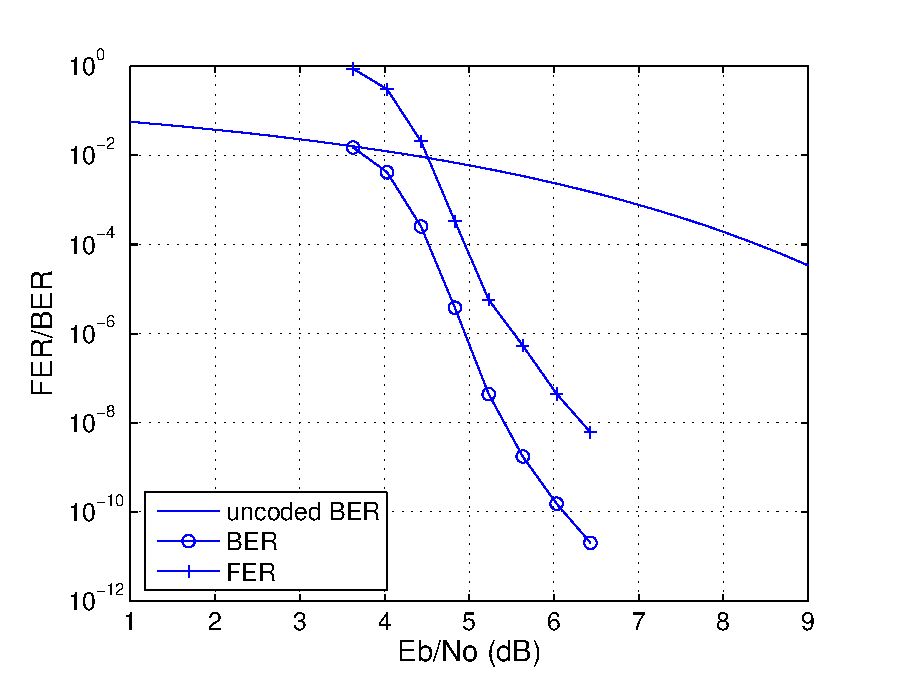
\includegraphics[keepaspectratio,width=4.5in]{474_lara3.eps}
\caption{Experimental Results for $C_{47,4}$} \label{expif}
\end{figure}

%\begin{figure}[h]
%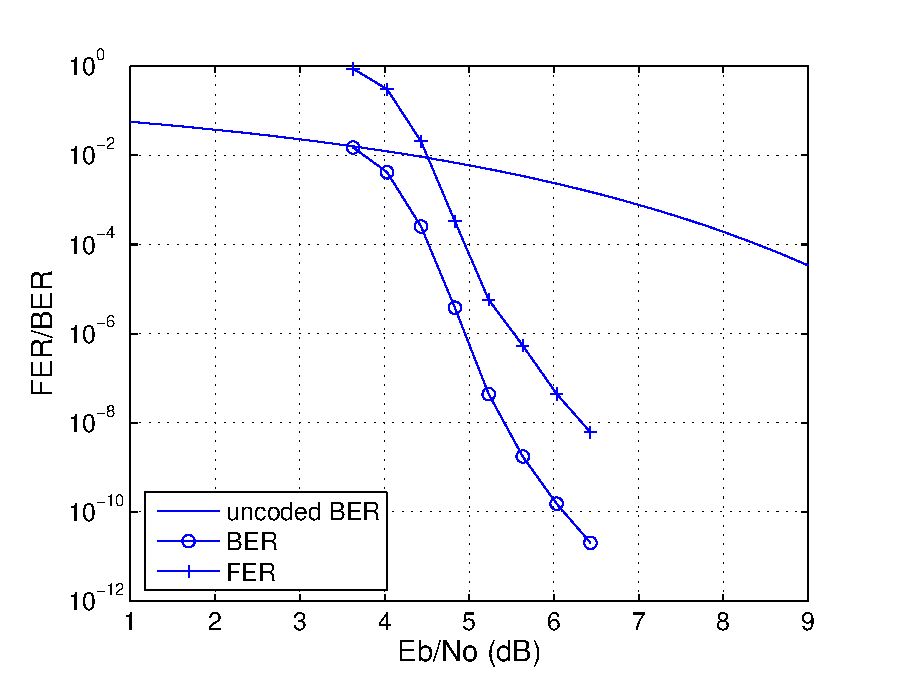
\includegraphics[keepaspectratio,width=4.5in]{474_lara3.eps}
%\caption{Experimental Results for $C_{41,4}$} \label{expif2}
%\end{figure}


\section{Summary and Concluding Remarks}

In this Chapter we presented a detailed analysis of the dominant
configurations in the error-floor regime of high rate array-based
LDPC codes. We provided an explicit description of the minimal
(fully) absorbing sets and showed the non-existence of certain
candidate configurations. We also enumerated minimal (fully)
absorbing sets and showed how their number scales with the
codeword length. Experiments on an emulation platform were
performed and were found to be in agreement with the theoretical
description of the dominant errors.
